%\documentclass[a4paper]{report}
\documentclass[openany]{book}
\newcommand{\rootpath}{../../..}
% --- Packages
\usepackage{amsmath}
\usepackage[a4paper]{geometry}
\geometry{verbose,tmargin=2cm,bmargin=2cm,lmargin=3cm,rmargin=3cm}
\usepackage{color}
\usepackage{comment}
%\usepackage{enumitem}
\usepackage[utf8]{inputenc}
\usepackage{fancyhdr}
\usepackage{float}
\usepackage{framed}
\usepackage{graphicx}
\usepackage[colorlinks = true,urlcolor  = blue]{hyperref}
\usepackage{listings}
\usepackage{makeidx}
\usepackage{markdown}
\usepackage{multirow}
\usepackage{subcaption}
\usepackage{subfiles}
\usepackage{tikz}
\usepackage{truncate}
\usepackage{xcolor}
\usepackage{xr}

% === Packages
 % Import packages
\newcommand{\ar}[1]{\index{to be checked}{\textcolor{blue}{AR:#1}}}
\newcommand{\BCFile}{description of the boundary type. This file is only used to generate the \file{geometry.geo} file.}
\newcommand{\BoussinesqMap}{spatial distribution of the Boussinesq coefficient~}
\newcommand{\CellPorosityMap}[1]{spatial distribution of the storage porosity in cells (#1 model)~}
\newcommand{\defaultvalue}[1]{\textit{\{Default value = #1}\}~}
\newcommand{\EdgePorosityMap}[1]{spatial distribution of the conveyance porosity along interfaces (#1 model)~}
\newcommand{\file}[1]{\textit{#1}}
\newcommand{\folder}[1]{\textit{#1}}
\newcommand{\Fr}{\mathrm{Fr}}
\newcommand{\FrictionStricklerMap}{spatial distribution of the Strickler coefficient~}
\newcommand{\GeometryFile}{geometry file~}
\newcommand{\h}{\mathrm{h}}
\newcommand{\HydroBCTimeSeries}{boundary condition time series~}
\newcommand{\InitialConditionsMap}{spatial distribution of the initial condition~}
\newcommand{\InputSWD}{input file~}
\newcommand{\keyword}[2]{\textbf{#1}=#2}
\newcommand{\MeshFile}{mesh. This file is only used to generate the \file{geometry.geo} file.~}
\newcommand{\m}{\mathrm{m}}
\renewcommand{\today}{\ifcase \month \or January\or February\or March\or April\or May \or June\or July\or August\or September\or October\or November\or December\fi, \number \year} 

% --- Lire et extraire la version ---
\newread\versionfile
\openin\versionfile=\rootpath/src/common/version.h
\read\versionfile to \linea
\read\versionfile to \lineb
\read\versionfile to \linec % cette ligne contient la version
\closein\versionfile
% Extraire le contenu entre guillemets
\def\extractversion#1"#2"#3\endextractversion{#2}
\edef\myversion{\expandafter\extractversion\linec\endextractversion}


\newcommand{\nodefaultvalue}{\textit{\{No default value}\}~}
\newcommand{\param}[1]{\textbf{#1}}
\newcommand{\pfg}[1]{\index{to be checked}{\textcolor{blue}{PFG:#1}}}
\newcommand{\Q}[1]{\textcolor{red}{\textbf{Q:} #1}}
\newcommand{\ResultBoundaryFluxes}{time series of the discharge crossing each type of boundary.~}
\newcommand{\ResultHydroFile}{hydrodynamic results at time XXX. XXX is the time from the beginning of the simulation using the ISO...\pfg{complete} format.~}
\newcommand{\rmk}{\index{remark}\textcolor{red}}
\newcommand{\s}{\mathrm{s}}
\newcommand{\swd}{SW2D}
\newcommand{\swConverter}{\emph{sw2dConverter\:}}
\newcommand{\swConverterReverse}{\emph{swConverterReverse\:}}
\newcommand{\swNSPreProcess}{\emph{sw2dNSPreProcess\:}}
\newcommand{\swOutputConverter}{\emph{swOutputConverter\:}}
\newcommand{\swPorosityMapper}{\emph{sw2dPorosityMapper\:}}
\newcommand{\swPostProcess}{\emph{sw2dPostProcess\:}}
\newcommand{\swSolver}{\emph{sw2dSolver\:}}
\newcommand{\swZone}{\emph{sw2dZone\:}}
\newcommand{\swdd}{SW2D~}

\newtheorem{remark}{Remark}


% --- Setup
\parindent 0pt % pas de retrait en début de paragraphe
 \hypersetup{
    pdfborderstyle={/S/U/W 1}, % underline links instead of boxes
    linkbordercolor=red,       % color of internal links
    citebordercolor=green,     % color of links to bibliography
    filebordercolor=magenta,   % color of file links
    urlbordercolor=blue        % color of external links
}
\definecolor{backcolour}{rgb}{0.95,0.95,0.92}
\lstdefinestyle{mystyle}{
    basicstyle=\ttfamily\small,
    backgroundcolor=\color{backcolour},
    breakatwhitespace=false,         
    breaklines=true,                 
    captionpos=b,   
    frame=single,
    keepspaces=true,                 
%    numbers=left,                    
%    numbersep=5pt,                  
    showspaces=false,                
    showstringspaces=false,
    showtabs=false,                  
    tabsize=2}
\lstset{style=mystyle}
\definecolor{lightgray}{gray}{0.9}
\newcommand{\inlinecode}[1]{\colorbox{backcolour}{\lstinline {#1}}}


\newcommand{\citeCode}[1]{\texttt{\zz#1\zz}}%In a perfect world, this would be changed to allow linebreaks anywhere in #1

\def\zz#1{%
 \ifx\zz#1\else
   #1\linebreak[1]\expandafter\zz
 \fi}

\externaldocument{../Guides/user/InputFile/input_sw2d}
\externaldocument{../Guides/user/InputFile/input_zone}
% === Setup   % Import macros
%%%
\newcommand\guide{User's Guide}
\newcommand\authors{Lilas Bugeau, Pascal Finaud-Guyot, Vincent Guinot, Antoine Rousseau}
\addtolength{\footskip}{20pt}
\pagestyle{fancy}

%%% 
\begin{document}

% Configure "fancy" style (applied to all pages)
\fancyhf{}
\fancyhead[LE]{\small\truncate{6cm}{\leftmark}}
\fancyhead[LO]{\small\truncate{6cm}{\rightmark}}
\fancyfoot[C]{\thepage}  % <-- numéro de page visible en bas

% Redefine plain (chapter start) to comply with "fancy"
%\fancypagestyle{plain}{%
%  \fancyhf{}
%  \fancyhead[LE]{\small\truncate{6cm}{\leftmark}}
%  \fancyhead[LO]{\small\truncate{6cm}{\rightmark}}
%  \fancyfoot[C]{\thepage}
%}
% Force plain (used at chapter beginning) to be equal to fancy
 \makeatletter
 \let\ps@plain\ps@fancy
 \makeatother

% Cadre décoratif avec TikZ
\thispagestyle{empty}
 \newgeometry{top=3cm,bottom=3cm,left=2.5cm,right=2.5cm}
    {\centering
    %\begin{tikzpicture}[remember picture, overlay]
        %\draw[line width=2pt, color=black] 
       %     ([xshift=1cm,yshift=-1cm]current page.north west) 
       %    rectangle 
       %    ([xshift=-1cm,yshift=1cm]current page.south east);
    %\end{tikzpicture}
    
    % Logo ou image
    \vspace*{1cm}
    \includegraphics[width=0.5\textwidth]{\rootpath/doc/common/figures/InrUM.png} 
    \vspace*{2cm}
    
    % Titre
    {\Huge {SW2D}}\\[.3cm]
    {\Large\bfseries \guide \\[0.5cm]}
    \rule{\linewidth}{0.5mm}
    % Sous-titre
    ~\\
    {\large Version \myversion}\\[0.5cm]
    {\large \today}\\[2cm]
    
        \vspace*{1cm}
    \includegraphics[width=0.4\textwidth]{\rootpath/doc/common/figures/logo_sw2d.png}
    \vspace*{2cm}
    
    % Auteur ou société
    \vfill
    \textsc{Main developers:}\\[0.3cm]
    {\Large \authors}\\[1cm]
    
    % Bas de page
    \vfill
    \rule{0.8\textwidth}{0.4pt}\\[0.3cm]
    {\small © 2025 Inria \& Université de Montpellier}
    \restoregeometry
    }
\pagebreak

\tableofcontents

\pagebreak

\fancyfoot[R]{SW2D \guide, version \myversion}
%%%

%%%
\chapter{Working environment \label{ch:workEnv}}
\input{./user/Simulation_Sequence}
\input{./user/Simulation_Structure}
%%% 
\chapter{Using \swConverter \label{ch:swConverter}}
\section{Invoking \swConverter}
NOTE: it is expected that the binary file \swConverter is in your path, so that it may be invoked from anywhere in your directories. If not, you will have to make sure that you enter the complete relative path to the \swConverter file. Do not hesitate to use SW2D shortcuts (see Chapter \ref{ch:shortcuts}).

The \swConverter executable is used as follows.

\begin{enumerate}
	\item Localize your project folder. This project folder must contain a subfolder named \texttt{primary\_files} with the following files
	\begin{itemize}
		\item (mandatory) \texttt{input.conv}
		\item (mandatory) a mesh file (.2dm is the only supported format at present)
		\item (optional) a Boundary Condition (BC) code file
	\end{itemize}
	\item Open a shell/prompt (command line window).
	\item Type
	\begin{verbatim}
	sw2dConverter.exe <path_to_project_folder>
	\end{verbatim}
	This results in the creation of the \texttt{input/geometry.sw2d} file.
	
	\remark{The path to your project folder is the relative path, starting from where the \swConverter command is called. In particular, if you are already at the root of your project folder, you may simply run the command 'sw2dConverter.exe .'}
	
\end{enumerate}

\input{./user/inputFile/swConverter_Input}
\section{Troubleshooting for \swConverter}

\paragraph*{The geometry.sw2d file cannot be created} 
\begin{itemize}
	\item Error message: \texttt{The file does not exist .\textbackslash [model\_name]\textbackslash input \textbackslash geometry.sw2d}
	\item Solution: The \textbackslash input folder does not exist within the directory structure. It must be created manually.		
\end{itemize}

\paragraph*{A procedure entry point cannot be found} 
\begin{itemize}
	\item Error message: \texttt{The procedure entry point  [usually a very long name] cannot be found in the dynamic link library}.
	\item Solution: 
	\begin{enumerate}
		\item Contact the SW2D team and ask for a static library install.
	\end{enumerate}
\end{itemize}


%%%
\chapter{Using \swConverterReverse \label{ch:swConverterReverse}}
\section{Invoking \swConverterReverse}

NB: The \swConverterReverse was coded in Python. It can be compiled into an executable file (using pyinstaller, for example), but by default, only the Python script is available. This chapter explains how to use this utility in both cases. \\
Note that you must have Python installed to run the Python script. \\

The \swConverterReverse is used to reconstruct the \swConverter's input files from a generated \file{geometry.sw2d} file.

\begin{enumerate}
	\item Localize your project folder. Make sure that the \file{geometry.sw2d} file is present in the \file{input} folder.
	\item Open a shell/prompt (command line window).
	\item \begin{itemize}
		\item If you have \swConverterReverse in the form of an executable file, type
		\begin{small}\begin{verbatim}
		sw2dConverterReverse <path_to_project_folder>
		\end{verbatim}\end{small}
		\item If you are using the python script, type
		\begin{small}\begin{verbatim}
		python <path_to_python_apps>/sw2dConverterReverse.py <path_to_project_folder>
		\end{verbatim}\end{small}
	\end{itemize}
	This results in the creation of \swConverter input files in the \file{log} folder : \file{input.conv}, \file{\textlangle filemane\textrangle.2dm}, and possibly \file{\textlangle filemane\textrangle.bc}.
\end{enumerate}

%%%
\chapter{Using \swNSPreProcess \label{ch:swNSPreProcess}}
\section{Invoking \swNSPreProcess}

NB: The \swNSPreProcess was coded in Python. It can be compiled into an executable file (using pyinstaller, for example), but by default, only the Python script is available. This chapter explains how to use this utility in both cases. \\
Note that you must have Python installed to run the Python script. \\

The \swNSPreProcess is used to create \file{input/qsections.txt} and \file{primary\_files/\textlangle filename\textrangle.bc}  files from the nodestrings defined in the \file{primary\_files/\textlangle filename\textrangle.2dm} file.
Each nodestring in the .2dm file is converted into a qesction and/or a boundary and written in the corresponding file(s).

\begin{enumerate}
	\item Localize your project folder. Make sure that the \file{NS\_conversion.txt} and \file{\textlangle filename\textrangle.2dm} files are present in the \file{primary\_files} folder.
	\item Open a shell/prompt (command line window).
	\item \begin{itemize}
		\item If you have \swNSPreProcess in the form of an executable file, type
		\begin{small}\begin{verbatim}
		sw2dNSPreProcess <path_to_project_folder> <destination_format>
		\end{verbatim}\end{small}
		\item If you are using the python script, type
		\begin{small}\begin{verbatim}
		python <path_to_python_apps>/sw2dNSPreProcess.py <path_to_project_folder> <destination_format>
		\end{verbatim}\end{small}
	\end{itemize}
	This results in the creation of two files: \begin{itemize}
		\item \file{primary\_files/\textlangle filename\textrangle.bc}, where \textlangle filename\textrangle  is the same as the .2dm file name
		\item \file{input/qsections.txt}
	\end{itemize}
\end{enumerate}

\input{./user/inputFile/swNSPreProcess_Input}
%%%
\chapter{Using \swZone \label{ch:swZone}}
\section{Invoking \swZone}
NOTE: it is expected that the binary file \swZone is in your path, so that it may be invoked from anywhere in your directories. If not, you will have to make sure that you enter the complete relative path to the \swZone file. Do not hesitate to use SW2D shortcuts (see Chapter \ref{ch:shortcuts}).

The \swZone executable is used to generate spatially distributed parameter files. Files \texttt{geometry.sw2d} and \texttt{input.zone} must be created before running this executable. It is run as follows.

\begin{enumerate}
	\item Navigate to the parent folder of the \swdd project folder.
	\item Make sure that the \texttt{input.zone} file is present in the \texttt{primary\_files} folder
	\item Open a shell/prompt (command line window).
	\item Type
	\begin{verbatim}
	sw2dZone.exe <path_to_project_folder>
	\end{verbatim}
	\item One or many text files for the spatially distributed parameters are generated in the \texttt{[model\_name]/input} folder. The name of these files are defined by the user in \texttt{input.zone}.
	\end{enumerate}

%%
%%
\section{File \texttt{input.zone}}
\subsection{Purpose}
This file is the main file controlling the \swZone executable. Its purpose is to create spatially distributed (cell- or edge-based) parameter files to be read as inputs by \swSolver. The parameters are assumed to be uniform within zones defined by polygons.
%
\subsection{Format description}
Empty lines or lines starting with hash '\#' or equal '=' signs are ignored. The spelling of the parameters is case sensitive.

This text file contains four mandatory blocks that are delimited by specific line strings.

\begin{scriptsize}
\begin{tabular}{l | l | l}
\hline
Block & starting line string & ending line string \\
\hline
Block 1 & \texttt{Block1: zones list BEGIN (compulsory line)} & \texttt{Block1: zones list END (compulsory line)} \\
Block 2 & \texttt{Block2: default parameter value BEGIN (compulsory line)} & \texttt{Block2: default parameter value END (compulsory line)} \\
Block 3 & \texttt{Block3: linking variable-zone BEGIN (compulsory line)} & \texttt{Block3: linking variable-zone END (compulsory line)} \\
Block 4 & \texttt{Block4: output file names BEGIN (compulsory line)} & \texttt{Block4: output file name END (compulsory line)} \\
\hline
\end{tabular}
\end{scriptsize}

\subsubsection{Block 1}
Each line of Block 1 defines one polygon. For each polygon, the summits can be either identified by their coordinates or as a node of the mesh. Each line should correspond to one of the two possible formats:
\begin{itemize}
    \item 
    \begin{lstlisting}
    <NAME> $P$ $x_1$ $y_1$ $x_2$ $y_2$ ... $x_i$ $y_i$ ... \end{lstlisting}
where \texttt{<NAME>} is the name of the zone, $P$ indicates that the summits are defined by physical coordinates, and the $x_i,y_i$ couples are the coordinates of the polynomial vertices.
    \item 
        \begin{lstlisting}
<NAME> $N$ $n_1$ $n_2$ ... $n_i$ ...
\end{lstlisting}
where \texttt{<NAME>} is the name of the zone, $N$ indicates that the summits are defined by mesh nodes, and the $n_i$ are the node identifiers for the vertices of the polynomial. The $n_i$ must therefore correspond to actual mesh node numbers.
\end{itemize}


\subsubsection{Block 2}
Each line of Block 2 defines the default value for each parameter. The format is the following
\begin{lstlisting}
<PARAM> <DEFAULT VALUE>
\end{lstlisting}
where \texttt{<PARAM>} is the name of the parameter and \texttt{<DEFAULT VALUE>} is the default value for this parameter. Note that
\begin{itemize}
\item SI units are used for all parameters
\item \swZone does not check whether the value is physically meaningful
\end{itemize}. 

\subsubsection{Block 3}
Each line in Block 3 assigns a numerical value to a parameter within a polygon previously defined in Block 1. The format is the following
\begin{lstlisting}
<PARAM> <VALUE> <NAME>
\end{lstlisting}
where \texttt{<PARAM>} is the name of the parameter, \texttt{<VALUE>} is its numerical value and \texttt{<NAME>} is the name of one of the polygons defined in Block 1. 

The parameters assigned in this Block 3 must have a default value defined in Block 2.

If two or more blocks overlap, the parameter values provided in the last polygon of the list will overwrite those previously defined in the overlapping area. 

\subsubsection{Block 4}
Each line in Block 4 defines the files to be created by \swZone and the parameters to be written into them. The format is the following
\begin{lstlisting}
<FILENAME> <PARAM_1> ... <PARAM_i> ...
\end{lstlisting}
where \texttt{<FILENAME>} is the output file name and \texttt{<PARAM\_i>} are the parameters to be written into this file. 

\subsection{Sample file}
In this sample file, the parameter file \texttt{initial\_conditions\_map.txt} is to be filled with three different parameters : h, q and v.
The default values for h, q and v are 50, 0.0 and -1.0 respectively.
A quadrangular polygon (called "Zone1") is defined by the coordinates of its vertices $(-1,-1), (400,-1),(400,1), (-1,1)$. Within this polygon, the parameter \texttt{h} is set to 10, while q and v are equal to their default values. 
A second polygon (called "Zone2") is defined as a draft (the \# character indicates that this is a comment line) using the Ids of its 7 vertices. 

\begin{verbatim}
= line of comments
# symbol to comment : (# =)
Block1: zones list BEGIN (compulsory line)
Zone1	P	-1	-1	400	-1	400	1	-1	1
#Zone2	N	1   2   3   4   5   8   12
Block1: zones list END (compulsory line)
Block2: default parameter value BEGIN (compulsory line)
h	50.
q	0.
v	-1.
Block2: default parameter value END (compulsory line)
Block3: linking variable-zone BEGIN (compulsory line)
h	10.	Zone1
Block3: linking variable-zone END (compulsory line)
Block4: output file name BEGIN (compulsory line)
initial_conditions_map.txt  h   q   v
Block4: output file name END (compulsory line)
\end{verbatim}
%%%
\chapter{Using \swPorosityMapper \label{ch:swPorosityMapper}}
\section{Invoking \swPorosityMapper}
NOTE: it is expected that the binary file \swPorosityMapper is in your path, so that it may be invoked from anywhere in your directories. If not, you will have to make sure that you enter the complete relative path to the \swPorosityMapper file. Do not hesitate to use SW2D shortcuts (see Chapter \ref{ch:shortcuts}).

The \swPorosityMapper binary file is used to generate porosity map files.
Files \texttt{input/geometry.sw2d}, \texttt{primary\_files/input.pmap} and \texttt{primary\_files/buildings.txt} must be created before running the mapper.
It is run as follows.

\begin{enumerate}
	\item Navigate to the parent folder of the \swdd project folder.
	\item Make sure that the \texttt{buildings.txt} file is present in the \texttt{primary\_files} folder
	\item Open a shell/prompt (command line window).
	\item Type
	\begin{verbatim}
	sw2dPorosityMapper.exe <path_to_project_folder>
	\end{verbatim}
	\item One or three text files are generated based on the porosity model : \texttt{<POROSITY>\_cell\_porosity\_map.txt} and possibly \texttt{<POROSITY>\_edge\_bnd\_porosity\_map.txt} and \texttt{<POROSITY>\_edge\_int\_porosity\_map.txt}, where \texttt{<POROSITY>} is the porosity model specified in \texttt{input.pmap}.
	\end{enumerate}

\section{File \texttt{input.pmap}}
\subsection{Purpose}
The text file \texttt{input.pmap} specifies how the \swPorosityMapper executable is to be run for generating the porosity maps. 

\subsection{Format description}
\texttt{input.pmap} is a text file. It contains one keyword per line, with format
\begin{lstlisting}
<KEYWORD> <VALUE>
\end{lstlisting}
The order of the keywords does not matter. Empty lines or lines starting with hash '\#' or equal '=' signs are considered as comment lines.\\
Note that
\begin{itemize}
\item The keywords and its value must be separated by at least one space or tabulation characters.
\item The spelling of the keywords is not case sensitive.\\
\item If a given keyword occurs several times in the file, the last read value overwrites the previously specified ones.
\item All physical parameters (e.g. gravitational acceleration, etc.) are in S.I. units.
\end{itemize}

\subsection{List of allowed keywords}

\begin{description}

\item[model] \defaultvalue{none} Set the porosity model used to generate the maps. Allowed values:
\begin{description}
\item[sp] Single Porosity model
\item[dip] Dual-Integral Porosity model
\item[ddp] Depth Dependant Porosity model
\end{description}

\item[input] \defaultvalue{footprint} Set the format expected from the input file \texttt{buildings.txt}. Allowed values:
\begin{description}
\item[footprint] The file specifies the building spatial footprints coordinates
\item[raster] The file consists in a Cartesian grid
\end{description}

\end{description}

\subsection{Example}
\begin{verbatim}
= ligne de commentaire
# symbole pour commentaire : (# =)
=== Porosity Mapper
model	dip
input	footprint
========
\end{verbatim}

%%
%%
\section{File \texttt{buildings.txt}}
\subsection{Purpose}
This file contains information regarding the position and height of the buildings, which is used by the mapper to compute the porosity of each cell and each edge.\\

There are two different possible formats for this file.
The used format is defined in \texttt{input.pmap}, the allowed values are \texttt{raster} and \texttt{footprint}.
They are both explained in the two following subsections.

\subsection{Format description: raster}
This format consists in a Cartesian grid based on (possibly irregular) $x-$ and $y-$coordinates (see Figure \ref{fig:porosity_mapping}).\\
%
The first line is the header containing "x    y    height".
Then, each line has the following format: 
\begin{lstlisting}
<x> <y> <h> \end{lstlisting}
where $x_i$ and $y_i$ are the coordinates of the $i^{th}$ point on the buildings grid and $h_i$ is the building height at that point.
\\
The file is organised so that the grid is scanned line by line, from top to bottom. The points are then arranged in descending order of y and in ascending order of x for each y.
In this way, we start with the points from $x_0$, $y_m$ to $x_n$, $y_m$, then those from $x_0$, $y_{m-1}$ to $x_n$, $y_{m-1}$, and so on.\\
The  \texttt{buildings.txt} is tested to make sure that $x-$ and $y-$coordinates are arranged as described above, but it is rather expected that this file is built from another tool (\textit{e.g.} raster). In particular this format does not correspond to a simple "1 line = 1 building" description. Again, the main reason is that the file is not expected to be hand-made. 

\begin{figure}[htbp]
    \centering
    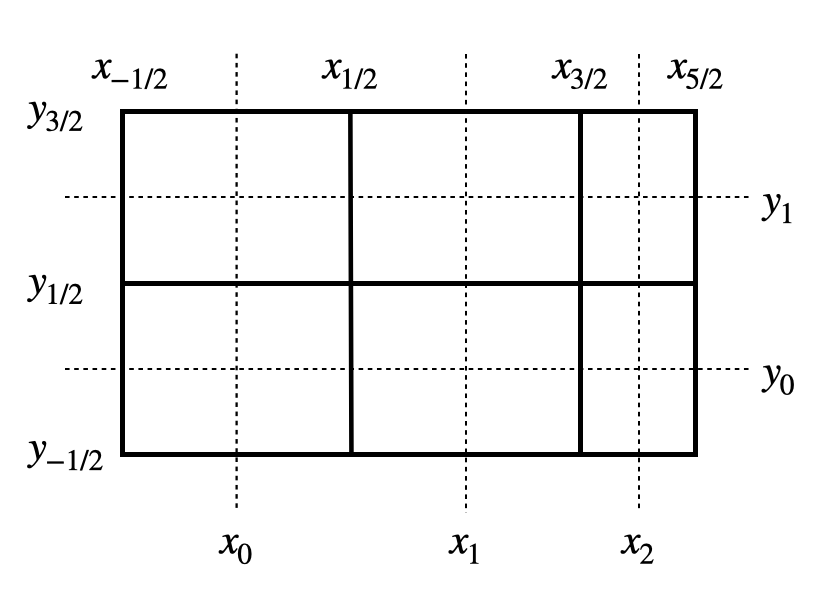
\includegraphics[width=0.5\textwidth]{../../common/figures/porosity_mapper.png}
    \caption{Cartesian grid for the definition of the \texttt{buildings.txt} file. In this case, the file should have 7 lines: header and 6 lines corresponding to each position ($x_i$, $y_j$). The $h$-value for each of theses positions corresponds to the building average height on the rectangle ($x_{i-1/2}$, $x_{i+1/2}$)$\times$($y_{i-1/2}$,$y_{i+1/2}$).}
    \label{fig:porosity_mapping}
\end{figure}

\subsection{Format description: footprint}
This format consists in a list of polygon coordinates corresponding to the building spatial footprints.

The first line is the header containing "x1 y1 … xn yn".
Then, each line describes one building has the following format:
\begin{lstlisting}
<x_1> <y_1> ... <x_i> <y_i> ... <-h> \end{lstlisting}
where $x_i$, $y_i$ are the coordinates of the $i^{th}$ vertice of the building footprint, and -h is optional and is the heigh of the building preceded by a minus sign (used for DDP).

% 
\chapter{Using \swSolver \label{ch:swSolver}}
\section{Invoking \swSolver}
NOTE: it is expected that the binary file \swSolver is in your path, so that it may be invoked from anywhere in your directories. If not, you will have to make sure that you enter the complete relative path to the \swSolver file. Do not hesitate to use SW2D shortcuts (see Chapter \ref{ch:shortcuts}).

The \swSolver executable is used as follows:

\begin{enumerate}
	\item Localize your project folder. This project folder must contain a subfolder named \texttt{input} with the minimum set of input files
	\item Open a shell/prompt (command line window).
	\item Type
	\begin{verbatim}
	sw2dSolver.exe <path_to_project_folder>
	\end{verbatim}
\end{enumerate}

\section{Minimal set of files and keywords for \swSolver}
Prior to running the \swSolver executable the user must make sure that the following minimal set of files is available.

\begin{enumerate}
	\item the \texttt{input.solv} simulation configuration file  (even if it is empty)
	\item the \texttt{geometry.sw2d} geometry file (produced but \swConverter)
	\item \texttt{initial\_conditions\_map.txt}
	\item \texttt{hydro\_boundary\_time\_series.txt}
\end{enumerate}
Besides, if specific models such as porosity-based models are activated, additional parameters may be required (porosity maps, etc.).
\begin{table}[H]
\index{Flie!input}
\begin{tabular}{p{7cm}| p{8cm}}
\hline
Model(s) & Required file(s) \\
\hline
model\_friction = chezy & friction\_chezy\_map.txt \\
\hline
model\_friction = manning & friction\_manning\_map.txt \\
\hline
model\_friction = strickler & friction\_strickler\_map.txt \\
\hline
model\_hyp = dip & Boussinesq\_map.txt \\
                 & DIP\_cell\_porosity\_map.txt \\
                 & DIP\_edge\_bnd\_porosity\_map.txt \\
                 & DIP\_edge\_int\_porosity\_map.txt \\
\hline
model\_hyp = sp & Boussinesq\_map.txt \\
                & SP\_cell\_porosity\_map.txt \\
\hline
model\_infiltration = horton & infiltration\_horton\_parameter\_map.txt \\
\hline
model\_runoff = infiltration\_coefficient & infiltration\_coefficient\_map.txt \\ 
      & precipitation\_station\_codes\_map.txt \\
\hline
model\_runoff = runoff\_coefficient & infiltration\_coefficient\_map.txt \\
                & precipitation\_station\_codes\_map.txt \\         
\hline
model\_singular\_head\_loss = active & singular\_head\_loss\_map.txt \\
\hline
\end{tabular}

\end{table}

\section{Time monitoring}
The \swSolver executable monitors the time spent on each step within the time loop sequence (i.e. between the first and last time steps in the simulation). Here is a typical console output

\begin{lstlisting}
[Info] Total clock time =  2.56636 
[Info] Hyperbolic time  =  1.41228  ( 55 % ) 
[Info]    - LRStates    =  0.403368  ( 15 % ) 
[Info]    - TimeStep    =  0.087421  ( 3 % ) 
[Info]    - Fluxes      =  0.147892  ( 5 % ) 
[Info]    - Balance     =  0.756254  ( 29 % ) 
[Info]    - Div. corr.  =  0.001173  ( 0 % ) 
[Info] Parabolic time  =  0.001153  ( 0 % ) 
[Info] Source time      =  0.074666  ( 2 % ) 
[Info] Storage time     =  1.05195  ( 40 % )
\end{lstlisting}

The breakdown is as follows.\\
\begin{tabular}{p{3cm} p{11cm}}
Total clock time & The total time spent between beginning and end of the time stepping process (model initialization is not included)\\
Hyperbolic time & Total time spent in the hyperbolic part of the simulation\\
\;\; --  LRStates & The time spent in the definition of the Riemann problems at the interfaces (hyperbolic model)\\
\;\; --  TimeStep & The time spent in computing the time step from CFL stability constraints (hyperbolic model)\\
\;\; --  Fluxes & The time spent to compute fluxes for the finite volume method (hyperbolic model)\\
\;\; --  Balance & The time spent to update state variables from the computed fluxes (hyperbolic model)\\
\;\; --  Div. corr & The time spent in bounding the velocity and Fr to physically acceptable values (hyperbolic model)\\
Parabolic time & Total time spent in the parabolic part of the simulation\\
Source time& The time spent in computing the effets of the source terms (friction, precipitation, wind stress, etc.)\\
Storage time& The time spent to store fields in output files
\end{tabular}


\hypertarget{InputSwddFormat}{}
\section{File \texttt{input.solv}}
\subsection{Purpose}
This file is the main file controlling the simulation. It defines the models that have to be used and the key parameters.

\subsection{Format description}
\texttt{<input.solv>} is a text file. It contains one keyword per line, with format
\begin{lstlisting}
<KEYWORD> <VALUE>
\end{lstlisting}
The order of the keywords does not matter. Empty lines or lines starting with hash '\#' or equal '=' signs are considered as comment lines.\\
Note that
\begin{itemize}
\item The keywords and its value must be separated by at least one space or tabulation characters.
\item Keywords spelling is not case sensitive.
\item If a given keyword occurs several times in the file, the last read value overwrites the previously specified ones.
\item All physical parameters (e.g. gravitational acceleration, etc.) are in S.I. units.
\end{itemize}

\subsection{List of allowed keywords}

\begin{description}
\begin{comment}
\item[compute\_hydro] \defaultvalue{compute}\index{transport!transport_hydro} specifies how the hydrodynamic fields are provided to the transport simulation. Allowed values:
\begin{description}
    \item[compute] compute hydrodynamics by solving the shallow water equations 
    \item[read] read hydrodynamic variables from a file \Q{dans ce cas, quel est le nom et le format de ce fichier?}
\end{description}

\item[contact\_ext\_margin] \defaultvalue{0.01}\index{transport!contact_ext_margin} set the buffer size for dealing with debris contact

\item[contact\_restitution] \defaultvalue{1}\index{transport!contact\_restitution} elastic coefficient for debris contact
\end{comment}


\item[cfl\_max] \defaultvalue{1}\index{Courant_number} defines the maximum permissible Courant/CFL number for timestep computation. Any strictly positive value may be specified. However, the CFL may be limited automatically to a maximum value ensuring stability depending on the \textbf{num\_scheme} used (e.g. 1 for the Godunov or MUSCL-EVR scheme).

\item [ddpDDP\_chi\_phi\_max]  \Q{Unknown parameter} \defaultvalue{20.0} upper bound for the ratio $\phi_\Omega / \phi_\Gamma$ in the Depth-Dependent Porosity (ddpDDP) closure model. Used only if \textbf{model\_hyperb = ddpDDP}.

\item [ddpDDP\_chi\_theta\_max]  \Q{Unknown parameter} \defaultvalue{20.0} upper bound for the ratio $\theta_\Omega / \theta_\Gamma$ in the Depth-Dependent Porosity (ddpDDP) closure model. Used only if \textbf{model\_hyperb = ddpDDP}.

\item [ddp\_ztab0\_log]  \Q{Unknown parameter} \defaultvalue{\texttt{no}} defines whether the lower elevations for the $\phi_\Gamma (z)$ and $\phi_\Omega (z)$ laws should be cast into a log file for further graphical display. The file is named \texttt{ddp\_zTab.txt}. Allowed values:
\begin{description}
\item [no] no file will be written. Any previously existing file in the \texttt{/log} folder will be erased.
\item [yes] the file will be written.
\end{description}
\textbf{NOTE} the $z-$ values cas in the file are the minimum values in the $\phi(z)$ laws. Denoting by $z_{\min,i}$ the lower point for the $\phi_\Gamma(z)$ law at Interface $i$, in the log file the elevation $z_{\min,i}$ is assigned to all the points of this interface. The same principle is retained for the cells. Therefore, the interfaces and cells appear horizontal in the log files. However, their elevations are only those of their lowest points.

\item[div\_corr] \defaultvalue{none}\index{Divergence correction}specifies whether divergence correction is to be activated. Allowed values:
\begin{description}
    \item[none] no divergence correction
    \item[limit\_flux]  prevents cell drying issues by reducing the divergence of numerical fluxes across the interfaces. This is an iterative process, requiring that the value for \param{n\_it\_div\_max} be set.
    \item[limit\_timestep] applies a reduction factor to the computation time step to avoid cell overdrying
\end{description}

\item[dt\_map](s) \defaultvalue{100}specifies the time interval for storing the hydrodynamic variables in the form of maps (in the \textbf{output} folder).
\begin{description}
	\item[Remark:] Additional map storage times that are not multiplae of \textbf{dt\_map} may be specified in a separate file, see Subsection \ref{sec:extraction_times_list}.
\end{description}

\item[dt\_max](s) \defaultvalue{10}specifies the maximum permissible computational timestep.

\item[dt\_time\_series](s) \index{Probes}\defaultvalue{100}specifies the time interval for pointwise storage of the results (at probes). This parameter is used as soon as the file \file{probe\_locations.txt} in the input folder is not empty (see Subsection \ref{sec:probe_locations}).

\item[fr\_max] \index{fr\_max}\defaultvalue{100} is the maximum permissible value for the Froude number Fr. Should Fr exceed this value at the end of a time step, the flow velocity is reduced such that $\max ||\mathbf{v}|| = \mathrm{fr\_max} \sqrt{gh}$.

\item[gravity] (ms$^{-2}$) \defaultvalue{9.81}specifies the value of the gravitational acceleration.

\item[h\_min] (m) \defaultvalue{$10^{-5}$}is a threshold depth. The mass and momentum fluxes between two adjacent cells are computed only provided that the water depth is larger than \param{h\_min} in at least one of the cells.
%%%%%\item[model\_building] \defaultvalue{none}\index{building}

%\item[hotstart\_time] (s) \defaultvalue{0}\index{hotstart}If defined, the initial conditions are read from a previously computed ResultHydro file. This file must be copied into the input folder and will supersede the initial conditions file. The value for hotstart\_time must correspond to the numerical value of the time present in the name of the ResultHydro file.  \Q{Not working yet (at least not this way).}

\item [log\_write] \defaultvalue{false} Specifies whether log files should be written in the log folder.
\begin{description}
\item [false] Log files will not be written (saves disk space in case of big meshes).
\item [true] Log files will be written at the end of the initialization stage.
\end{description}

%\item[model\_building] \defaultvalue{none}\index{Source term!Building}sets how buildings are accounted for. Allowed values:
%\begin{description}
%    \item[none] no building effect computed
%    \item[cell\_average] individual buildings are not represented but the cell average effect is accounted
%\end{description}

\item[model\_friction] \defaultvalue{none}\index{Friction} specifies the bottom friction model. Allowed values:
\begin{description}
    \item[none] no friction model
    \item[chezy] \index{Friction!Chezy} Chezy's model is used. Requires the additional map file \file{input/friction\_chezy\_map.txt}.
    \item[manning] \index{Friction!Manning}the Manning formulation is used. Requires the additional map file \file{input/friction\_manning\_map.txt}.
    \item[strickler] \index{Friction!Strickler}friction is modelled using Strickler's model. Requires the additional map file \file{input/friction\_strickler\_map.txt}.
\end{description}

%%%%%\item[model\_gates] \defaultvalue{none}\index{gates}

\item[model\_hyperb] \defaultvalue{none}\index{Model!Hyperbolic}Specifies the hyperbolic model. Allowed values:
\begin{description}
%    \item[ddpDDP]  \Q{Unknown parameter}\index{Model!Hyperbolic!ddpDDP}Depth-Dependent Porosity model (ddpDDP). Requires additional files \texttt{Boussinesq\_map.txt}, \texttt{ddpDDP\_cell\_porosity\_map.txt}, \texttt{ddpDDP\_edge\_porosity\_map.txt}. See also keywords \textbf{ddpDDP\_chi\_phi\_max} and \textbf{ddpDDP\_chi\_theta\_max}
   
  %  \item[dip]  \Q{Unknown parameter}\index{Model!Hyperbolic!DIP}Dual-Integral Porosity model. Requires the files \texttt{DIP\_cell\_momentum\_dissipation\_map.txt}, \texttt{DIP\_cell\_porosity\_map.txt}.
  \item [liswes]  \index{Model!Hyperbolic!LISWES} Local Inertial Shallow water model  
   \item[sp]  \index{Model!Hyperbolic!SP}Single Porosity model.
    \item[swes] \index{Model!Hyperbolic!SWES}Shallow water model.
\end{description}
%
\item [model\_infiltration] \defaultvalue{none}\index{Source term!infiltration}
sets how infiltration is modelled. Allowed values:
\begin{description}
	\item [none] No infiltration.
	\item [h\_proportional]. The infiltration rate in a given cell is equal to $k$ times the water depth. Required file: \texttt{infiltration\_parameter\_map.txt} that provides the cellwises $k$ values.
	\item [horton]. The infiltration rate is equal to $I_c$, the soil infiltration capacity, as long as the water depth is non-zero. Required file: \texttt{infiltration\_parameter\_map.txt} that provides the cellwise $I_c$ values.
\end{description}
%
\item [model\_momentum\_diffusion] \defaultvalue{none} \index{Model!Parabolic!Momentum diffusion}
Defines how momentum diffusion is to be accounted for.
\begin{description}
\item [none] No momentum diffusion
\item [velocity\_independent] The momentum diffusion coefficient is constant in space and time. Its numerical value is specified with the keyword \textbf{momentum\_diffusion\_coefficient}.
\end{description}
%
\item [model\_momentum\_diffusion\_coefficient] \defaultvalue{$10^{-6}$} \index{Model!Parabolic!Momentum diffusion}
The numerical value of the momentum diffusion coefficient, in m$^2$s$^{-1}$.
%
%

\item[model\_momentum\_dissipation] \defaultvalue{none}\index{Source term!momentum dissipation}defines if the momentum dissipation is accounted. Allowed values:
\begin{description}
    \item[none] no momentum dissipation
    \item[active] momentum dissipation is accounted for. In this case, the file \texttt{DIP\_cell\_momentum\_dissipation\_map.txt} must be provided in the \texttt{input} folder.
\end{description}
%
%
\item [model\_porosity\_rainfall] \defaultvalue{water\_only} \index{Source term!rainfall!porosity}
defines how the rainfall source term is accounted for in porosity models. Allowed values:
\begin{description}
	\item [everywhere] the rain is assumed to fall onto 100 \% of the computational cells. The rain falling onto the solid phase (fraction $1 - \phi$ of the cell area, where $\phi$ is the storage porosity) is routed instantaneously to the water phase. This amounts to multiplying the rainfall intensity onto the water phase (fraction $\phi$) by $1/\phi$. In the cells where $\phi = 0$, the rainfall contribution is zero.
	\item [water\_only] the rain is assumed to fall only onto the fraction of the cell occupied by water. The rain falling onto the emerged topography is assumed to infiltrate instantaneously and is not accounted for in the water balance.
\end{description}
%
\item[model\_runoff] \defaultvalue{none}\index{Source term!runoff}
sets how the rain is accounted for in the runoff generation process. Allowed values:
\begin{description}
    \item [none] no runoff generation
    \item [full\_rainfall] 100 \% of the rainfall intensity falling onto a given cell is converted to runoff.
    \item[infiltration\_coefficient] rainfall is accounted for. On each cell, the amount of runoff is the rainfall multiplied by (1 -- infiltration\_coefficient). The following files are required:
    \begin{itemize}
    	\item \texttt{precipitation\_station\_codes\_map.txt}
    	\item \texttt{precipitation\_time\_series.txt}
    	\item \texttt{infiltration\_coefficient\_map.txt}
	\end{itemize}     
    \item[runoff\_coefficient] rainfall is accounted for. On each cell, the amount of runoff is the rainfall multiplied by runoff\_coefficient. The following files are required:
    \begin{itemize}
    	\item \texttt{precipitation\_station\_codes\_map.txt}
    	\item \texttt{precipitation\_time\_series.txt}
    	\item \texttt{runoff\_coefficient\_map.txt}
	\end{itemize}     
     \item[scs] rainfall is accounted for. The runoff is computed from the scs parameters. The following files are required:
    \begin{itemize}
    	\item \texttt{precipitation\_station\_codes\_map.txt}
    	\item \texttt{precipitation\_time\_series.txt}
    	\item \texttt{scs\_parameter\_map.txt}
\end{itemize}     

\end{description}

%


\item[model\_singular\_headloss] \defaultvalue{none}\index{Source term!singular headloss}sets how the singular headloss are accounted. Allowed values:
\begin{description}
    \item[none] no singular headloss computed
     \item[active] singular headloss computed
\end{description}

%\item[model\_logjam] \defaultvalue{none}\index{Transport!logjam}sets the model for log transport. Allowed values:
%\begin{description}
%    \item[none] no log transport computed
%\end{description}

%\item[model\_transport\_reaction] \defaultvalue{none}Not used yet


\item[model\_wind] \defaultvalue{none}\index{Source term!Wind}sets how the wind effect is computed. Allowed values:
\begin{description}
    \item[none] no wind effect computation
    \item[smithbanke] \index{Source term!Wind}wind effect computation using Smith \& Banke's model.
\end{description}

\item[negative\_depth\_detection] \defaultvalue{none}specifies whether the simulation should stop when the water depth becomes negative in at least one of the cells. 
\begin{description}
	\item [none] the computation will not be stopped if a negative depth is computed in one of the cells at the end of the hyperbolic time step.
	\item [active] the computation will be stopped as soon as the water depth is negative in at least one cell at the end of the hyperbolic time step.
\end{description}
Note: the occurrence of negative depths can be reduced using the divergence correction function (see \param{div\_corr}).


\item[n\_it\_div\_max] \defaultvalue{0}\index{Divergence correction}  sets the maximal number of iterations allowed in the divergence correction process. This parameter is used only if the parameter \param{div\_corr} is set to limit\_flux.

\item[num\_scheme] defines the numerical scheme used to compute the hyperbolic part of the equation. Default and other possible values depend on the hyperbolic model:

\begin{tabular}{p{3cm}|p{3cm}|p{7cm}}
\hline
\param{model\_hyperb} keyword & default value for \param{num\_scheme} & allowed values for \param{num\_scheme} \\
\hline
\hline
ddp  & godunov & godunov \\
\hline
dip  & godunov & godunov \\
\hline
sp   & godunov & godunov \\
\hline
swes & godunov & godunov, muscl\_evr\\
\hline
\end{tabular}\\

\item[output\_format] \defaultvalue{all}defines whether output should be written in text or binary files. Allowed values:
\begin{description}
     \item[all] both txt and bin files are generated
     \item[bin] only bin files are generated
     \item[txt] only bin files are generated
\end{description}

\item[phi\_min] (m) \defaultvalue{same as small\_real ($10^{-16}$)} is a threshold on phi. The mass and momentum fluxes between two adjacent cells are computed only provided that the phi is larger than \param{phi\_min} in at least one of the cells.

\item[q\_section] \defaultvalue{0}defines if qsection fluxs are computed.
If this option is ativated \file{qsection.txt} must exist in the \file{input} folder.
It results in the creation of \file{output/qsection.txt} Allowed values:
\begin{description}
    \item[0] no q sections
    \item[1] read q sections from \file{input/qsection.txt} and write fluxes into \file{output/qsection.txt}
\end{description}

\item[store\_flag] \defaultvalue{default}defines stored variables in hydrodynamics results maps.  Allowed values: 
\begin{description}
\item [none] Nothing is stored in the output files
\item [default] The minimal sel of variables to reconstruct all other variables is stored: $x,y,z_b,$ + conserved variables
\item[all] As default + additional variables (hydraulic head, flow velocity, Froude number, CFL, etc.)
\end{description}

The list of stored variables depends on the hyperbolic model.

\item[t\_0] (s) \defaultvalue{0} Starting time of the simulation. 

\item[t\_max] (s) \defaultvalue{100}Ending time of the simulation.

\item[topo\_discretization] \defaultvalue{discontinuous}. Defines how the topographical source term is to be discretized in the SWES, SP and DIP models. 
Allowed values:
\begin{description}
\item [blending] The source term is discretized as a mixture between a piecewise constant topography and a continuous one. The blending between these two discretizations is a continuous, linear function of the ratio of the surface to bottom gradient.
\item [discontinuous] The source term is discretized on the assumption of a piecewise constant cell bottom elevation.
\end{description}


\begin{comment}

\item[verb\_algo\_timestep]  \defaultvalue{0} controls the degree of verbosity of the CFL-based time step limitation. For \textbf{algo\_timestep} $\ge 2$, the Id of the limiting cell and its flow variables are stored in the log file.

\item[verb\_map\_boussinesq] \index{Boussinesq}\defaultvalue{1}specifies if the Boussinesq coefficients map used in the computation has to be written (0: no / $>0$: yes) in \file{log/boussinesq.txt}. Note that this option will be disregarded when model\_hyperb = swes because this model does not use the Boussinesq coefficient.

\item[verb\_map\_init\_cond] \index{Initial conditions}\defaultvalue{1}specifies if the initial conditions map used in the computation has to be written (0: no / $>0$: yes) in \file{log/initial\_conditions\_map.txt}.

\item[verb\_map\_porosity] \defaultvalue{1} \index{Porosity}\defaultvalue{1}specifies if the porosity values maps used in the computation have to be written (0: no / $>0$: yes). The files generated depend also on the user-defined hyperbolic model:\\

\begin{tabular}{c|c}
\hline
\param{model\_hyperb} keyword & files generated \\
\hline
\hline
\multirow{3}{*}{ddpDDP} & \file{ddpDDP\_debug.txt} \\
                     & \file{ddpDDP\_PhiG.txt} \\
                     & \file{ddpDDP\_PhiW.txt} \\
\hline                     
\multirow{2}{*}{dip} & \file{DIP\_PhiG.txt} \\
                     & \file{DIP\_PhiW.txt} \\
\hline                     
sp   & \file{SP\_PhiW.txt} \\
\hline                     
swes &  none \\
\hline                     
\end{tabular}

\item[verb\_process\_ddpDDP] \defaultvalue{0}specifies the level of verbosity for all ddpDDP model-specific computations. The bigger the value, the more verbosity you get (0 = no verbosity).

\item[verb\_process\_friction] \defaultvalue{0}specifies the level of verbosity of the friction computation function. The bigger the value, the more verbosity you get (0 = no verbosity) NOT IMPLEMENTED

\item[verb\_process\_hyperb] \defaultvalue{0}specifies the verbosity level for of the functions computing the hyperbolic part. The higher the value, the stronger the verbosity (0 = no verbosity)

\item[verb\_process\_momentum\_diff] \defaultvalue{0}  NOT IMPLEMENTED

\item[verb\_process\_overall] \defaultvalue{0}specifies the level of verbosity of the main workflow. The higher the value, the stronger the verbosity (0 = no verbosity).

\item[verb\_process\_velocity\_corr] \defaultvalue{0}  NOT IMPLEMENTED

\item[verb\_properties\_cells] \defaultvalue{1}specifies if the cells properties have to be written (0: no / $>0$: yes) in \file{log/cells.txt}.

\item[verb\_properties\_interfaces] \defaultvalue{1}specifies if the interfaces properties have to be written (0: no / $>0$: yes) in \file{log/interfaces.txt}.

\item[verb\_properties\_nodes] \defaultvalue{1}specifies if the nodes properties have to be written (0: no / $>0$: yes) in \file{log/nodes.txt}.

\end{comment}

\item[vmax] (ms$^{-1}$) \defaultvalue{100} specifies the maximum permissible velocity. Should $||\mathbf{v}||$ exceed this value at the end of a time step, the flow velocity is reduced such that $\max ||\mathbf{v}|| = \mathbf{vmax} $.



%%%%\item[verb\_process\_velocity\_corr] \defaultvalue{0} NOT USED
\end{description}

\subsection{Example}
\begin{verbatim}
= unread line
# sign to comment a full line : (# =)
=== Model
model_hyperb	dip
num_scheme	godunov
tmax	100.
dt_max	1.5
dt_map	10.
dt_time_series	15.
========
model_friction	chezy
========
\end{verbatim}
This chapter describes the format of the parameter files in the \file{input} folder.

\section{Input files for spatially distributed parameters (in ./input)}
%
\subsection{Compulsory maps required by models}
\index{Input maps}
%
Hereafter is a list of the map files required by the various hyperbolic models. \\
\begin{tabular}{l|l}
\hline
model\_hyp = dip & initial\_conditions\_map.txt \\
                 & DIP\_cell\_porosity\_map.txt \\
                 & DIP\_edge\_porosity\_map.txt \\
\hline 
model\_hyp = liswes & initial\_conditions\_map.txt \\
\hline 
model\_hyp = sp & initial\_conditions\_map.txt \\
                & SP\_cell\_porosity\_map.txt \\
\hline 
model\_hyp = swes & initial\_conditions\_map.txt \\
\hline
\end{tabular}
\input{./user/inputFile/Boussinesq_map.tex}
\input{./user/inputFile/Buildings_exchange_map.tex}
% -- REMOVE FOR PARTNERS
\subsection{DDP\_cell\_porosity\_map.txt}
\index{Model!Hyperbolic!DDP}\label{sec_Model!Hyperbolic!DDP!cellPorosityMap}
\subsubsection{Purpose}
The Depth-Dependent Porosity (DDP) model requires that the variations in the storage porosity $\phi_\Omega$ with the water depth be specified on a cell-by-cell basis. This is the domain-based $\phi_\Omega(z)$ law in the original publication \cite{Guinot_al_2018}.
The code provides 5 types of pre-defined law:
\begin{itemize}
    \item Law type -2: the porosity law is specified as a sequence of couples $(z_i, \phi_i$), where the $z_i$ are ranked in ascending order. The $z_i$ are relative to the ground surface elevation, that is computed from the 2D mesh. The $z_i$ are the levels used in the tabulation of the law.
    \item Law type -1: the porosity law is specified as a sequence of couples $(z_i, \phi_i$), where the $z_i$ are ranked in ascending order. The $z_i$ are relative to the ground surface elevation, that is computed from the 2D mesh. The law is later tabulated using \textbf{ntabmax} intermediate levels between $z_1$ and $z_N$.
    \item Law type 0: the porosity law is specified by a sequence of elevations $(z_1, \ldots, z_N)$ in ascending order. The porosity is piecewise constant, equal to $i/N$ between $z_i$ and $z_i+1$ and to unity above $z_N$.  The $z_i$ are relative to the ground surface elevation as in Law type -1.
    \item Law type 1: the porosity is zero below an elevation $z_1$ relative to the ground elevation, and equal to $\phi_1$ above. 
    \item Law type 2: the porosity varies linearly from $\phi_1$ to $\phi_2$ between elevations $z_1$ and $z_2$ relative to the ground surface. It is zero below $z_1$ and $\phi_2$ above $z_2$.
    \item Law type 3: the porosity varies linearly from $\phi_1$ to $\phi_2$ between elevations $z_1$ and $z_2$ relative to the ground surface. It is zero below $z_1$ and $\phi_3$ above $z_2$.
\end{itemize}
If the laws are spatially distributed, each cell may obey a different law type.
%
\subsubsection{Law type specification format}
Five porosity law types are allowed in the current version of the software.\\

\begin{tabular}{p{1.5cm} | p{5.5cm} | p{8cm}} 
\hline
Law type & Parameters to be provided in file (separated using \texttt{<Tab>} characters) & Comments \\
\hline
\hline
-2 & -1 $N$ $\phi_1 \: z_1  \ldots \phi_N \: z_N$ &  $N$: number of $(z,\phi)$ couples. \\
\hline
-1 & -1 $N$ $\phi_1 \: z_1  \ldots \phi_N \: z_N$ &  $N$: number of $(z,\phi)$ couples. \\
\hline
0 & 0 $N$ $z_1 \ldots z_N$ & $N$ : number of points in the $\phi(z)$ law. $z_i$ : elevations relative to the ground level , by ascending order. \\
\hline
 1 & 1 $z_1$ $\phi_1$ & $z_1$: altitude (relative to local bottom elevation) above which $\phi=\phi_1$; $\phi = 0$ for $z < z_1$ \\
 \hline
 2 & 2 $z_1$ $z_2$ $\phi_1$ $\phi_2$ & Porosity $\phi$ is zero below $z_1$, varies linearly from $\phi_1$ to $\phi_2$ between $z_1$ and $z_2$, is equal to $\phi_2$ for $z > z_2$  \\
 \hline
 3 & 3 $z_1$ $z_2$ $\phi_1$ $\phi_2$ $\phi_3$ & Porosity $\phi$ is zero below $z_1$, varies linearly from $\phi_1$ to $\phi_2$ between $z_1$ and $z_2$, is equal to $\phi_3$ for $z > z_2$ \\
\hline
\end{tabular}
%
\subsubsection{Input file format}
%
File format for a uniform parameter set.  \texttt{\textbf{Bold}} : keyword, must appear as such in the file. \texttt{<Tab>}: tabulation character. \\
    \begin{tabular}{p{6cm} | p{9cm}}
    \hline
    Field(s) & Comment(s) \\
    \hline  \hline
    \texttt{\textbf{Unif} <Tab> \textbf{1}} & Flag is 1 because the parameter set is uniform \\ \hline
    \texttt{\textbf{NtabMax} <Tab> NtabMax} & NtabMax is the number of vertical discretization levels used for the $\phi_\Omega$(z) law \\ \hline
    \texttt{\textbf{==== Default Param}} & Section separator line, leave unchanged \\  \hline
    \texttt{\textbf{Uniform parameter set}} & Comment line, leave unchanged \\  \hline
    Parameter set     & The parameter set should obey the format given in the previous table \\ \hline
    \texttt{\textbf{==== Distrib}} & Section separator line, leave unchanged \\  \hline
    \end{tabular}
%
\vspace{10mm} \\
%
File format for a spatially distributed parameter set.  \texttt{\textbf{Bold}} : keyword, must appear as such in the file. \texttt{<Tab>}: tabulation character. \\
    \begin{tabular}{p{6cm} | p{9cm}}
    \hline
    Field(s) & Comment(s) \\
    \hline  \hline
    \texttt{\textbf{Unif} <Tab> \textbf{0}} & Flag is 0 because the parameter set is spatially variable \\ \hline
    \texttt{\textbf{NtabMax} <Tab> NtabMax} & NtabMax is the number of vertical discretization levels used for the $\phi_\Omega$(z) law \\ \hline
    \texttt{\textbf{==== Default Param}} & Section separator line, leave unchanged \\  \hline
    \texttt{\textbf{Uniform parameter set}} & Comment line, leave unchanged \\  \hline
    Parameter set     & The parameter set should obey the format given in the previous table \\ \hline
    \texttt{\textbf{==== Distrib}} & Section separator line, leave unchanged \\  \hline
    Parameter set [i]     & Parameter set, provided on a cell-by-cell basis. Index i runs sequentially from 1 to the number of cells. The parameter set should obey the format given in the Law type specification format table \\ \hline
    \end{tabular}
%
\subsubsection{Sample files}
%
\paragraph*{Example\#1: Uniform law type 2}
The porosity varies linearly from $\phi_1=0.$ to $\phi_2=1.$ between $z_1=3$ m and $z_2=10$ m.
\begin{verbatim}
Unif	1
NtabMax	50
==== Default Param
Type	Parameters(type)
2	3.	10.	0.	1.
==== Distrib
\end{verbatim}
%
\paragraph*{Example\#2: Distributed law type}
There are 3 cells in the model, the law types for cells 1, 2 and 3 are respectively 1, 0 and -1. The law type 0 in Cell 2 is given by 5 elevations. The Law type -1 in Cell 3 uses 2 $(z,\phi)$ couples.
\begin{verbatim}
Unif	0
NtabMax	50
==== Default Param
Type	Parameters(type)
2	3.	10.	0.	1.
==== Distrib
Type	Parameters(type)
1   2.3 0.5
0   5   0.1 0.4 0.7 1.2 2.5
-1  2   0.1 0.3 2.7 0.95
\end{verbatim}
\subsection{DDP\_edge\_porosity\_map.txt}\label{sec_Model!Hyperbolic!DDP!edgePorosityMap}
\index{Model!Hyperbolic!DDP}
\subsubsection{Purpose}
The Depth-Dependent Porosity (DDP) model requires that the variations in the connectivity porosity $\phi_\Gamma$ with the water depth be specified on an interface-per-interface basis. This is the domain-based $\phi_\Gamma(z)$ law in the original publication \cite{Guinot_al_2018}.
The code provides 5 types of pre-defined law. They are described in Subsection \ref{sec_Model!Hyperbolic!DDP!cellPorosityMap}.
%
\subsubsection{Format description}
The format is exactly the same as that of the cell porosity map, see \ref{sec_Model!Hyperbolic!DDP!cellPorosityMap}. The only difference is that the running index i goes from 1 to the number of interfaces (not the number of cells).
\subsubsection{Sample files}
See Subsection \ref{sec_Model!Hyperbolic!DDP!cellPorosityMap}.
\subsection{cell\_momentum\_dissipation\_map.txt}\label{sec_Model!Hyperbolic!cellMomentumDissipationMap}
\index{Model!Hyperbolic!DIP}
\subsubsection{Purpose}
The Dual Integral Porosity (DIP) model requires that the momentum dissipation tensor $\mu$ be specified on a cell-by-cell basis \cite{Guinot_al_2017}. This tensor is characterised by the momentum disspation coefficients $(\mu_1,\mu_2)$ in two orthogonal principal directions and the angle $\alpha_\mu$ between the 1st principal direction and the $x-$ axis.
%
\subsubsection{Input file format}
%
File format for a uniform tensor.  \texttt{\textbf{Bold}} : keyword, must appear as such in the file. \texttt{<Tab>}: tabulation character. \\
    \begin{tabular}{p{6cm} | p{9cm}}
    \hline
    Field(s) & Comment(s) \\
    \hline  \hline
    \texttt{\textbf{Unif} <Tab> \textbf{1}} & Flag is 1 because the tensor is uniform \\ \hline
    \texttt{\textbf{==== Default Param}} & Section separator line, leave unchanged \\  \hline
    \texttt{\textbf{mu1}  \textbf{mu2}  \textbf{alphamu}} & Comment line, leave unchanged \\  \hline
    $\mu_1 \quad \mu_2 \quad \alpha_\mu$      & The uniform values for $(\mu_1, \mu_2, \alpha_\mu)$ \\ \hline
    \texttt{\textbf{==== Distrib}} & Section separator line, leave unchanged \\  \hline
    \end{tabular}
%
\vspace{10mm} \\
%
File format for a spatially distributed parameter set.  \texttt{\textbf{Bold}} : keyword, must appear as such in the file. \texttt{<Tab>}: tabulation character. \\
    \begin{tabular}{p{6cm} | p{9cm}}
    \hline
    Field(s) & Comment(s) \\
    \hline  \hline
    \texttt{\textbf{Unif} <Tab> \textbf{0}} & Flag is 0 because the tensor is spatially distributed \\ \hline
    \texttt{\textbf{==== Default Param}} & Section separator line, leave unchanged \\  \hline
    \texttt{\textbf{PhiW}} & Comment line, leave unchanged \\  \hline
    \texttt{dummy  dummy dummy}     & These 3 values are ignored because \texttt{Flag} = 1 \\ \hline
    \texttt{\textbf{==== Distrib}} & Section separator line, leave unchanged \\  \hline
     $\mu_1 \quad \mu_2 \quad \alpha_\mu$      &  $(\mu_1, \mu_2, \alpha_\mu)_i$, provided on a cell-by-cell basis (1 line per cell). Index $i$ is the index of the cell in the mesh.  \\ \hline
    \end{tabular}
%
\subsubsection{Sample files}
%
\paragraph*{Example\#1: Uniform dissipation tensor}
Momentum dissipation coefficients in the principal directions are 0.25 and 0.10 respectively. The angle of the 1st principal direction with the $x-$
axis is 10 degrees.
\begin{verbatim}
Unif	1
==== Default Param
mu1		mu2	alpha_mu
0.25	0.10	10.0
==== Distrib
\end{verbatim}
%
\paragraph*{Example\#2: Distributed storage porosity}
There are 3 cells in the model. Cells 1 to 3 have the same dissipation coefficients, but the angle of the 1st principal direction increases from 10 to 30 degrees from Cell 1 to Cell 3.
\begin{verbatim}
Unif	0
==== Default Param
PhiW
0. 0.	0.
==== Distrib
0.25	0.10	10.0
0.25	0.10	20.0
0.25	0.10	30.0
\end{verbatim}

\input{./user/inputFile/dip/DIP_cell_porosity_map.tex}
\input{./user/inputFile/dip/DIP_edge_porosity_map.tex}
\input{./user/inputFile/sp/SP_cell_porosity_map.tex}
% == REMOVE FOR PARTNERS
\input{./user/inputFile/sourceTerms/Friction_Chezy_map.tex}
\input{./user/inputFile/sourceTerms/Friction_Manning_map.tex}
\input{./user/inputFile/sourceTerms/Friction_Strickler_map.tex}
\input{./user/inputFile/sourceTerms/Infiltration_coefficient_map.tex}
\input{./user/inputFile/sourceTerms/Infiltration_h_proportional_parameter_map.tex}
\input{./user/inputFile/sourceTerms/Infiltration_horton_parameter_map.tex}
\input{./user/inputFile/Initial_conditions_map.tex}
\input{./user/inputFile/sourceTerms/Precipitation_station_codes_map.tex}
\subsection{runoff\_coefficient\_map.txt}
\index{Source term!Infiltration}
\subsubsection{Purpose}
This file is required when \textbf{model\_runoff} is set to \textbf{runoff\_coefficient}. In this case, the runoff rate $R$ is computed from the precipitation rate $P$ as
\begin{equation}
R = (1 - R_c) P
\end{equation} where $R_c \in [0, 1]$ is the runoff coefficient. The spatial distribution for $R_c$ must be provided.
%
\subsubsection{Format description}
File format for a uniform $R_c$.  
\texttt{\textbf{Bold}} : keyword, must appear as such in the file. \texttt{<Tab>}: tabulation character. \\
    \begin{tabular}{p{6cm} | p{9cm}}
    \hline
    Field(s) & Comment(s) \\
    \hline  \hline
    \texttt{\textbf{Unif} <Tab> \textbf{1}} & Flag is 1 because $R_c$ is uniform \\ 
    \hline
    \texttt{\textbf{==== Default Param}} & Section separator line, leave unchanged \\
    \hline
    \texttt{\textbf{Infiltration\_coeff}} & Comment line, leave unchanged \\  
    \hline
    \texttt{k} & The uniform value for $R_c$ (dimensionless, between 0 and 1) \\ 
    \hline
    \texttt{\textbf{==== Distrib}} & Section separator line, leave unchanged \\  
    \hline
    \end{tabular}
%
\vspace{10mm} \\
%
File format for a spatially distributed $R_c$.  
\texttt{\textbf{Bold}} : keyword, must appear as such in the file. \texttt{<Tab>}: tabulation character. \\
    \begin{tabular}{p{6cm} | p{9cm}}
    \hline
    Field(s) & Comment(s) \\
    \hline  \hline
    \texttt{\textbf{Unif} <Tab> \textbf{0}} & Flag is 0 because $R_c$ is spatially variable \\ 
    \hline
    \texttt{\textbf{==== Default Param}} & Section separator line, leave unchanged \\ 
    \hline
    \texttt{\textbf{Infiltration\_coeff}} & Comment line, leave unchanged \\ 
    \hline
    \texttt{k}     & This value will be ignored because \texttt{Flag} = 1 \\ 
    \hline
    \texttt{\textbf{==== Distrib}} & Section separator line, leave unchanged \\  
    \hline
    \texttt{k[i]}      & Values for $R_c$ (dimensionless, between 0 and 1), provided on a cell-by-cell basis. Index i is the index of the cell in the mesh.  \\ 
    \hline
    \end{tabular}

\paragraph*{Sample file}
For a spatially ditributed coefficient.

\begin{verbatim}
Unif	0
==== Default Param
runoff_coefficient
0.8
==== Distrib
0.72
0.85
0.35
\end{verbatim}
\subsection{scs\_parameter\_map.txt}
\index{Source term!Infiltration}
\subsubsection{Purpose}
This file is required when \textbf{model\_runoff} is set to \textbf{scs}. In this case, the runoff rate $R$ is computed from the SCS formula
\begin{equation}
R = \frac{\max^2(P - I_a, 0}{\max(P - I_a, 0) + S}
\end{equation} where $I_a, S$ are recpectively the initial accumulation and soil storage capacity. The spatial distribution for these two parameters must be provided.
%
\subsubsection{Format description}
File format for a uniform $(I_a, S)$.  
\texttt{\textbf{Bold}} : keyword, must appear as such in the file. \texttt{<Tab>}: tabulation character. \\
    \begin{tabular}{p{6cm} | p{9cm}}
    \hline
    Field(s) & Comment(s) \\
    \hline  \hline
    \texttt{\textbf{Unif} <Tab> \textbf{1}} & Flag is 1 because $(I_a, S)$ is uniform \\ 
    \hline
    \texttt{\textbf{==== Default Param}} & Section separator line, leave unchanged \\
    \hline
    \texttt{\textbf{Ia <Tab> S}} & Comment line, leave unchanged \\  
    \hline
    \texttt{k} & The uniform values for $I_a$ and $S$ (positive, in m) \\ 
    \hline
    \texttt{\textbf{==== Distrib}} & Section separator line, leave unchanged \\  
    \hline
    \end{tabular}
%
\vspace{10mm} \\
%
File format for a spatially distributed $R_c$.  
\texttt{\textbf{Bold}} : keyword, must appear as such in the file. \texttt{<Tab>}: tabulation character. \\
    \begin{tabular}{p{6cm} | p{9cm}}
    \hline
    Field(s) & Comment(s) \\
    \hline  \hline
    \texttt{\textbf{Unif} <Tab> \textbf{0}} & Flag is 0 because $(I_a, S)$ is spatially variable \\ 
    \hline
    \texttt{\textbf{==== Default Param}} & Section separator line, leave unchanged \\ 
    \hline
    \texttt{\textbf{Ia <Tab> S}} & Comment line, leave unchanged \\ 
    \hline
    \texttt{k}     & This value will be ignored because \texttt{Flag} = 1 \\ 
    \hline
    \texttt{\textbf{==== Distrib}} & Section separator line, leave unchanged \\  
    \hline
    \texttt{Ia[i] <Tab> S[i]}      & Values for $I_a$ and $S$ (in m, positive), provided on a cell-by-cell basis. Index i is the index of the cell in the mesh.  \\ 
    \hline
    \end{tabular}

\paragraph*{Sample file}
For a spatially ditributed model.

\begin{verbatim}
Unif	0
==== Default Param
I_a		S  
0.02	0.1
==== Distrib
0.03	0.07
0.01	0.05
0.009	0.07
\end{verbatim}
\input{./user/inputFile/Singular_head_loss_map.tex}
\input{./user/inputFile/sourceTerms/Wind_station_codes_map.tex}

\section{Input files for time series (in ./input)}

%
\input{./user/inputFile/Hydro_boundary_time_series.tex}
\input{./user/inputFile/sourceTerms/Precipitation_time_series.tex}
\input{./user/inputFile/sourceTerms/Wind_time_series.tex}
\section{Miscellaneous input files}
%
\subsection{extraction\_times\_list.txt}\label{sec:extraction_times_list}
\index{Probes}
\subsubsection{Purpose}
This file specifies additional storage times in the form of maps. These are extra storage times that do not replace the \textbf{dt\_map}-periodic storage times specified in the input.solv file.
%
\subsubsection{Format description}
\begin{tabular}{p{5cm} | p{10cm}}
\hline
Field(s) & Format \\
\hline
\hline
\texttt{\# < text >} & Any line starting with the \texttt{\#} character are considered as comment lines and will be ignored \\
\hline
$t_1$ \texttt{name}$_1$ & extra map storage time \#1, followed by its label. The label will be appendend to the name of the map file created for this specific storage time. The time and the label must be separated by at least one space character (DO NOT USE TABs) \\
\hline
$\cdots$ & \\
\hline
$t_1$ \texttt{name}$_1$ & extra map storage time \#1, followed by its label. The label will be appendend to the name of the map file created for this specific storage time. The time and the label must be separated by at least one space character (DO NOT USE TABs) \\
\hline
\end{tabular}
%
\subsubsection{Example}
In the file hereafter, 4 additional storage times are requested.
\begin{verbatim}
#
# sample extractions times for specific data extractions
#

# Time   Extra label inserted in map file name
11.2 extra_time_11.2s
24. extra_time_24.0s
17.4 extra_time_17.4s
# comment line, insert as many as you like

# Blank lines like above will be ignored
22 extra_time_22s
\end{verbatim}

\hypertarget{ProbeLocationFileFormat}{}
\subsection{probe\_locations.txt}\label{sec:probe_locations}
\index{Probes}
\subsubsection{Purpose}
This file specifies the locations at which the flow variables are to be stored at the pre-defined \textbf{dt\_time\_series} time interval.
%
\subsubsection{Format description}
\begin{tabular}{p{5cm} | p{10cm}}
\hline
Field(s) & Format \\
\hline
\hline
\texttt{x  y  name} & This is the header line. The string \texttt{x  y  name} must be inserted without modification \\
\hline
$x_1 \; y_1$ \texttt{name}$_1$ & $x$ and $y$ coordinates (in m) of the 1st probe and its name, separated by at least one space character \\
\hline
$\cdots$ & \\
\hline
$x_N \; y_N$ \texttt{name}$_N$ & $x$ and $y$ coordinates (in m) of the $N$th probe and its name, separated by at least one space character \\
\hline
\end{tabular}
%
\subsubsection{Example}
In the file hereafter, there are 4 probes
\begin{verbatim}
x	y	name
50	0	probe_1
150	0	probe_2
350	0	probe_3
450	0	probe_4
\end{verbatim}
\subsection{\label{sec:qsection}qsection.txt}
%
\subsubsection{Purpose}
This file is used to specify the sections over which the fluxes are to be computed during the simulation.
A qsection is made up of all the edges associated with the same qsection name.

For each edge, the order in which the nodes are specified affects the result: when an edge is defined from its south node to its north node, a positive discharge crosses the edge from west to east.

%
\subsubsection{Format specification}
\begin{footnotesize}
\begin{tabular}{p{4cm} | p{10cm} }
\hline
Field(s) & Specification \\
\hline
\hline
$N$ & number of edges in the present file \\
\hline
$b_1 \rightharpoonup e_1 \rightharpoonup name_1$ &
\begin{itemize}
\item [$b_1$] Id of the beginning node of the 1st edge
\item [$e_1$] ID of the end node of the 1st edge in the file
\item [$name_1$] name of the 1st qsection
\item [$\rightharpoonup$] Tabulation character or space
\end{itemize} \\
\hline
$\vdots$ & (repeat) \\
\hline
$b_N \rightharpoonup e_N \rightharpoonup name_M$ & 
\begin{itemize}
\item [$b_N$] Id of the beginning node of the $N$th edge
\item [$e_N$] ID of the end node of the $N$th edge in the file
\item [$name_M$] name of the $M$th qsection
\end{itemize} \\
\hline
\end{tabular}
\end{footnotesize}

%
\subsubsection{Sample file}
In the following file, the first 5 edges are part of q section names qsection\_1, while the remaining 5 are part of q section names qsection\_2. 
\begin{verbatim}
10
1995	1741	qsection\_1
1741	1742	qsection\_1
1742	1743	qsection\_1
1743	1744	qsection\_1
1744	1745	qsection\_1
1745	1746	qsection\_2
1746	1747	qsection\_2
1747	1938	qsection\_2
1938	1939	qsection\_2
1939	1940	qsection\_2
\end{verbatim}
\hypertarget{RatingCurveBoundaryFormat}{}
\subsection{Hydro\_boundary\_rating\_curve.txt}
\index{Boundary}
\subsubsection{Purpose}
This file is made to prescribe the rating-curve type boundary conditions for hydrodynamics (number, type and values). These conditions come in addition to time series boundary condition.
%
\subsubsection{Input file format}
 \begin{tabular}{p{6cm} | p{9cm}}
    \hline
    Field(s) & Comment(s) \\
    \hline  \hline
    \texttt{\textbf{\#Comment   } } & Comment line, could be changed but not removed \\ \hline
    \texttt{\begin{tabular}{l}Description of the rating curve \\ bc\_code	-3 \\ type	interp \\	z0	0.4 \\\emph{LINE 5}\\ \emph{LINE 6}\end{tabular}
} & each rating curve $\Rightarrow$ 1 block of 6 lines.
    \begin{itemize}
    \item Line 1 : Comment line for the rating curve description, could be changed but not removed
		\item Line 2 : keyword \emph{bc\_code}: code of the boundary corresponding to the code assigned by the converter (see section \ref{sec:bc_file_format})
    \item Line 3 : keyword \emph{type}: type of the rating curve (allowed types, see below)
    \item Line 4 : keyword \emph{z0}: minimal elevation of the rating curve \emph{i.e.} if the water level within the cell is below than $z_0$ then the discharge is nil.
    \item Line 5 and Line 6 : depend of the type of rating curve
    \end{itemize} \\ \hline
	\end{tabular}  
\\
~\\ 
\paragraph{allowed types of rating curves}
\begin{description}
\item [interp] unit discharge is interpolated based on the water level $z$ within the cell using a curve $\left(z_{val}; q_{val}\right)$. If $z \le z_0$, the discharge is nil and if $z > \max\left(z_{val,i}\right)$, the unit-discharge is interpolated linearly based on the two last used-defined values (see figure below). The user has to define $\left(h_{val}; q_{val}\right)$ on line 5 and line 6 with $z_{val} = z_0 + h_{val}$.


 \begin{tabular}{p{5cm} | p{8.5cm}}

    \hline
    Field(s) & Comment(s) \\
    \hline  \hline
    \texttt{h\_val	0.00	0.50	1.00	1.50} & \begin{itemize}\item Line 5 : keyword \emph{h\_val} followed by a list of (positive and increasing) values of $h$. \end{itemize} \\
		\texttt{q\_val	0.00	0.07	0.20	0.37} & \begin{itemize}\item Line 6 : keyword \emph{q\_val} followed by a list of (positive) values of $q$. The lists $h_{val}$ and $q_{val}$ should contains the same number of values. By convention, the discharge is leaving the domain at a rating curve (thus negative) but the value are defined positively (the minus sign is added within the program). \end{itemize} \\
		\end{tabular}
		\\
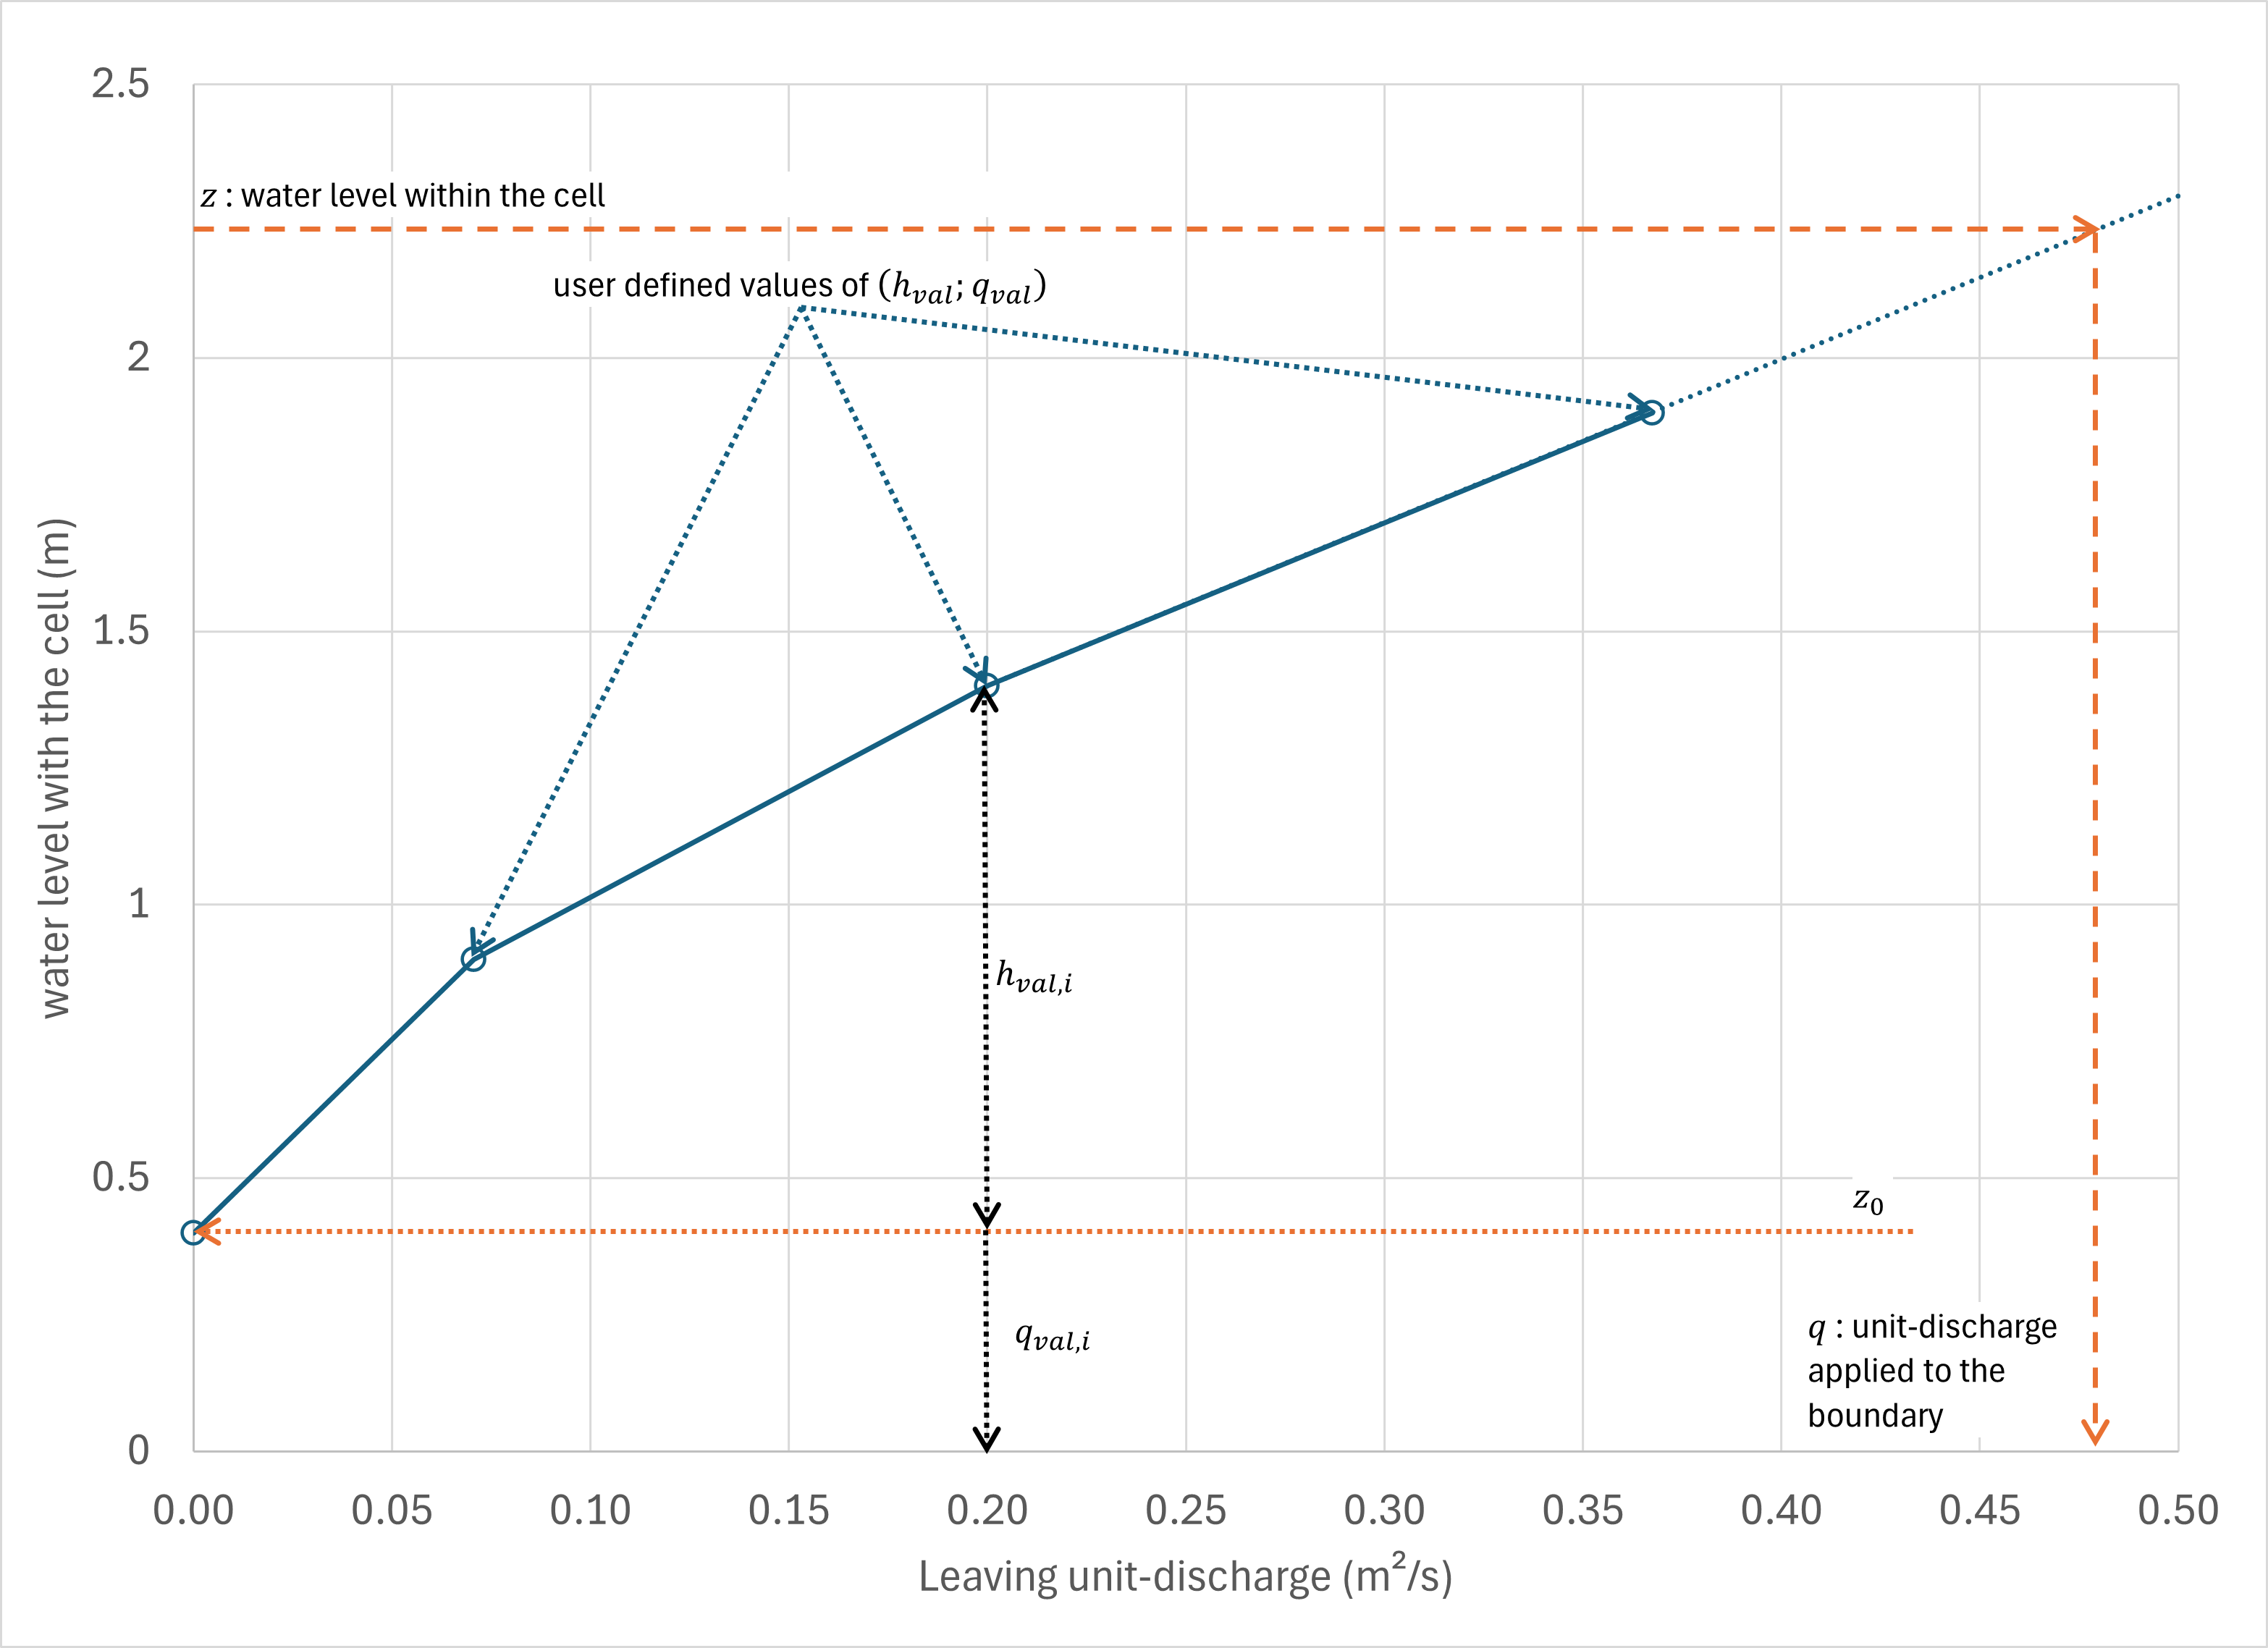
\includegraphics[width=0.7\columnwidth]{user/inputFile/RatingCurve.png}
		
\item [powerlaw] unit discharge is computed based on a powerlaw equation based on the water level $z$ within the cell:
\begin{subequations}\begin{eqnarray}
q = 0 & \texttt{if }  z < z_0 \\
q = a \left(z - z_0\right) ^ b & \texttt{otherwise}
\end{eqnarray}\end{subequations}

The user has to define the values of $a$ and $b$ on line 5 and line 6.


 \begin{tabular}{p{5cm} | p{8.5cm}}

    \hline
    Field(s) & Comment(s) \\
    \hline  \hline
    \texttt{a	0.20} & \begin{itemize}\item Line 5 : keyword \emph{a} followed by a positive number. By convention, the discharge is leaving the domain at a rating curve (thus negative) but the value of $a$ is defined positively (the minus sign is added within the program).\end{itemize} \\
		\texttt{b	1.5} & \begin{itemize}\item Line 6 : keyword \emph{b} followed by a non-nil number.  \end{itemize} \\
\end{tabular}
To avoid computational problems, the absolute value of $a$ and $b$ have to be greater than the program precision (defined to $10^{-16}$).
\end{description}   


		
%    
\subsubsection{Sample files}
\paragraph*{Example \#1}
Here, three rating curves are defined (with codes -2, -5 and -4). Defining three rating curve does not prevail that they will be used during the computation. If the bc\_code -5 has not be defined in the converter step (see section \ref{sec:bc_file_format}), the corresponding rating curve will be ignored.
\begin{verbatim}
\# each rating curve = 1 commented line (# or =) using followed by 5 lines containing the data (1st line is Always skipped)
\# 1st rating curve
bc_code	-2
type	interp
z0	0.4
h_val	0.00	0.25	0.50	0.75	1.00	1.25	1.50	1.75
q_val	0.00	0.125	0.354	0.650	1.000	1.398	1.837	2.315
\# 2nd rating curve
bc_code	-5
type	powerlaw
z0	0.4
a	0.44
b	2.50
\# 3rd rating curve
bc_code	-4
type	interp
z0	0.4
h_val	0.00	0.25	0.50
q_val	0.000	0.0125	0.0354
\end{verbatim}

%\section{output/ResultHydro.slf}\label{sec:selafin_output}

\subsection{Purpose}
When the \param{output\_slf} option is activated in the input file \texttt{input.solv}, the file \texttt{ResultHydro.slf} stores in a different format the same results as the \texttt{ResultHydro\_pDDDDdHHhMMmSSsXXX.txt} files, with the same variables and the same time step.\\

The selafin format allows all the time steps to be contained in one file and the results to be displayed in a temporal view in QGIS.\\

As selafin format cannot handle mixed meshes, to activate the \param{output\_slf} option, all the cells in the mesh must have the same number of edges. Otherwise, the code will return an error.

\subsection{Use}

To view the results in selafin format, follow the steps below:
\begin{itemize}
    \item Open the \texttt{ResultHydro.slf} file in QGIS
    \item Import only the mesh layer
    \item Activate the time controller panel
    \item Set the start and end times: the start time is the current date at 00:00 and the end time is the start date + simulation time. The time step must also be adapted to the simulation time step.
    \item Start the time display with the pause button or drag the cursor to navigate through the time steps.
\end{itemize}

% \subsection{Example}
% \begin{verbatim}
    
% \end{verbatim}
\section{Output files (in ./output)}
%
\subsection{ResultHydro\_pDDDDdHHhMMmSSsXXX.txt}\label{resulsubt_hydro_txt}

\subsubsection{Purpose}
This file stores the hydrodynamic results every \param{dt\_map}. To avoid any computational timestep reduction to store the results precisely every \param{dt\_map}, the results are stored when \pfg{explain algorithm}. The stored variables depend upon the chosen hyperbolic model (defined by the parameter \param{model\_hyperb}) and the \param{storeflag} parameter:
\begin{center}
\begin{tabular}{c|c|c}
\multirow{2}{*}{\param{model\_hyperb}} & \multicolumn{2}{c}{\param{storeflag} value} \\
& default & all \\
\hline
ddp  &  &  \\
dip  &  &  \\
sp   &  &  \\
swes & $h, \overrightarrow{q}$ & $h, \overrightarrow{q}, z, \overrightarrow{u}, \mathrm{Fr}, H_s, H_t, CFL$
\end{tabular}
\pfg{complete}
\end{center}

For vectorial fields, three values are stored in each cell: the two horizontal component of the vector and the vector norm.

\begin{center}
\begin{tabular}{c|l|c}
Symbol & Variable & Type of field \\
\hline
$CFL$ & cfl & scalar \\
$\mathrm{Fr}$ & froude & scalar \\
$h$ & water\_depth & scalar \\
$H_s$ & specific\_head & scalar \\
$H_t$ & total\_head & scalar \\
$\overrightarrow{q}$ & unit\_discharge\_x, unit\_discharge\_y and	unit\_discharge\_norm & vectorial \\
$\overrightarrow{u}$ & velocity\_x,	velocity\_y	and velocity\_norm & vectorial \\
$z$ & surface\_elevation & scalar
\end{tabular}
\end{center}

\subsubsection{Format description}
The precise simulation time for storing the variables is indicated in the file name using the ISO 8601 format. The file name is \file{ResultHydro\_pDDDDdHHhMMmSSsXXX.txt} where \emph{pDDDDdHHhMMmSSsXXX} is the elapsed time from the beginning of the simulation:
\begin{itemize}
    \item DDDD is the number of days (always on 4 digits)
    \item HH is the number of hours (always on 2 digits)
    \item MM is the number of minutes (always on 2 digits)
    \item SS is the number of seconds (always on 2 digits)
    \item XXX is the number of milliseconds (always on 3 digits)
\end{itemize}

% \subsection{Example}
% \begin{verbatim}
    
% \end{verbatim}
\subsection{ResultBoundaryFluxes.txt}
%
\subsubsection{Purpose}
This file stores the instantaneous discharge crossing each boundary every \param{dt\_time\_series}. In case of the boundary is composed of several edges, the stored discharge is the sum of the discharge crossing each edge. As the unit vector normal to the boundary edges is oriented from the exterior to the interior, a positive discharge enters the domain.
%
\subsubsection{Format description}
\texttt{<Tab>}: tabulation character. \\
    \begin{tabular}{p{6cm} p{9cm}}
    \hline
    \texttt{time <Tab> BC\_$x_1$ <Tab> \ldots <Tab> BC\_$x_N$} & This is the header line. $x_1$, \ldots, $x_N$ represent the boundary numbers as defined in the \file{2dm} file \\
    \hline 
    $t$ \texttt{<Tab>} $Q_1$ \texttt{<Tab>} \ldots \texttt{<Tab>} $Q_N$ & $t$ is the stored time, $Q_i$ is the discharge (in $\mathrm{m^3.s^{-1}}$) through the boundary $x_i$ \\
    \hline
    \ldots & one line per stored time \\ \hline
    \end{tabular}
%
\subsubsection{Example}
\begin{verbatim}
time	BC_1	BC_2	BC_3
2.0000000000e+1	0.0000000000e+0	4.3274586317e+1	-1.4193271476e+1
3.0000000000e+1	0.0000000000e+0	4.3149535653e+1	-1.4227591312e+1
4.0000000000e+1	0.0000000000e+0	4.3074013841e+1	-1.4246148173e+1
5.0000000000e+1	0.0000000000e+0	4.3030038602e+1	-1.4258119344e+1
6.0000000000e+1	0.0000000000e+0	4.3000513361e+1	-1.4266604580e+1
\end{verbatim}
\subsection{ProbeTimeSeries.txt}

\subsubsection{Purpose}
This unique text file stores the hydrodynamic time series for all probes identified in the \file{input/probes\_lacation.txt}. For every probe, 4 fields are stored: $z_b$, $h$, $q$ and $r$ (bottom elevation, water height, unit discharge in both $x-$ and $y-$directions. 

\subsubsection{Format description}
The file starts with 1 line for each probe: each lines contains the probe name, its $x-$ and $y-$ coordinates (these parameters are given by the user through the input file \file{input/probes\_lacation.txt}).\\
Then comes the header line (indicating the name of subsequent fields).\\
Finally, the following lines are dedicated to the output of time and for each probe, bottom elevation, water height, unit discharge in both $x-$ and $y-$directions. Each line thus contains $4n+1$ fields where $n$ is the number of probes.

\begin{tabular}{p{5cm} | p{10cm}}
\hline
Field(s) & Format \\
\hline
\hline
\hline
\texttt{name}$_1\;$ $x_1 \; y_1$  & name, $x-$ and $y-$coordinates (in m) of the 1st probe, separated by at least one space character \\
\hline
$\cdots$ & \\
\hline
\texttt{name}$_n\;$ $x_n \; y_n$  & name, $x-$ and $y-$coordinates (in m) of the $n$th probe, separated by at least one space character \\
\hline
\texttt{x  y  name} & This is the header line. The string \texttt{x  y  name} must be inserted without modification \\
\hline
$t_0\;$ $z_{b_1 }\; h_1 \; q_1 \; r_1 $ $\cdots$ $z_{b_n }\; h_n \; q_n \; r_n $ & initial time time, then for every probe: bottom elevation, water height, unit discharge in both $x-$ and $y-$directions, separated by at least one space character \\
\hline
$\cdots$ & (one lime every \param{dt\_time\_series}) \\
\hline
$t_f\;$ $z_{b_1 }\; h_1 \; q_1 \; r_1 $ $\cdots$ $z_{b_n }\; h_n \; q_n \; r_n $ & final time, then for every probe: bottom elevation, water height, unit discharge in both $x-$ and $y-$directions, separated by at least one space character \\
\hline
\end{tabular}
%
\subsubsection{Example}
In the file hereafter, there are 2 probes
\begin{small}
\begin{verbatim}
pr_1	6.0000000000e-01	4.0000000000e-01
other_probe	1.0000000000e+00	0.0000000000e+00
time	pr_1_zb	pr_1_h	pr_1_q	pr_1_r 	other_probe_zb 	other_probe_h	other_probe_q	other_probe_r
0.0000e+00	0.0000e+00	5.0000e+00	0.0000e+00	0.0000e+00	0.0000e+00	5.0000e+00	0.00000e+00	0.0000e+00
1.0000e+00	0.0000e+00	4.9000e+00	4.9926e-02	-3.6509e-16	0.0000e+00	4.9000e+00	4.99266e-02	-3.6509e-16	
\end{verbatim}
\end{small}
\subsection{qsection.txt}
%
\subsubsection{Purpose}
This file stores the instantaneous discharge crossing each qsection every \param{dt\_time\_series}. 
For each Q Section, the stored discharge is the sum of the discharge crossing each of its edges.
When an edge is defined in the input file from its south node to its north node, a positive discharge crosses the edge from west to east.
%
\subsubsection{Format description}
\texttt{<Tab>}: tabulation character. \\
    \begin{tabular}{p{6cm} p{9cm}}
    \hline
    \texttt{time <Tab> name\_1 <Tab> \ldots <Tab> name\_N} & This is the header line. \texttt{name\_1}, \ldots, \texttt{name\_N} represent the q section names as defined in the \file{input/qsection.txt} file \\
    \hline 
    $t$ \texttt{<Tab>} $Q_1$ \texttt{<Tab>} \ldots \texttt{<Tab>} $Q_N$ & $t$ is the stored time, $Q_i$ is the discharge (in $\mathrm{m^3.s^{-1}}$) through the q section \texttt{name\_i} \\
    \hline
    \ldots & one line per stored time \\ \hline
    \end{tabular}
%
\subsubsection{Example}
\begin{verbatim}
time	qsection_1	qsection_2	qsection_3
2.0000000000e+1	0.0000000000e+0	4.3274586317e+1	-1.4193271476e+1
3.0000000000e+1	0.0000000000e+0	4.3149535653e+1	-1.4227591312e+1
4.0000000000e+1	0.0000000000e+0	4.3074013841e+1	-1.4246148173e+1
5.0000000000e+1	0.0000000000e+0	4.3030038602e+1	-1.4258119344e+1
6.0000000000e+1	0.0000000000e+0	4.3000513361e+1	-1.4266604580e+1
\end{verbatim}


\chapter{Using \swOutputConverter \label{ch:swOutputConverter}}
\section{Invoking \swOutputConverter}

NB: The \swOutputConverter was coded in Python. It can be compiled into an executable file (using pyinstaller, for example), but by default, only the Python script is available. This chapter explains how to use this utility in both cases. \\
Note that you must have Python installed to run the Python script. \\

The \swOutputConverter is used to convert an output file \file{ResultHydro.bin} into other file formats.\\

\begin{enumerate}
	\item Localize your project folder. Make sure that the \file{ResultHydro.bin} file is present in the \file{output} folder.
	\item Open a shell/prompt (command line window).
	\item \begin{itemize}
		\item If you have \swOutputConverter in the form of an executable file, type
		\begin{small}\begin{verbatim}
		sw2dOutputConverter <path_to_project_folder> <destination_format>
		\end{verbatim}\end{small}
		\item If you are using the python script, type
		\begin{small}\begin{verbatim}
		python <path_to_python_apps>/sw2dOutputConverter.py <path_to_project_folder> <destination_format>
		\end{verbatim}\end{small}
	\end{itemize}
	This results in the creation of result file(s) in the desired format in the \file{output} folder. Possible formats are : \texttt{text}, \texttt{netCDF}.
\end{enumerate}

If specified format is \texttt{text}, the created files are the ones described in Section \ref{result_hydro_txt}. Else the format is specified in the following subsection.
\section{output/ResultHydro.nc}

The \texttt{ResultHydro.nc} file stores the simulation results in a netCDF file.
As for the \texttt{ResultHydro.bin} file, all the time steps are contained in one file.
This specific format allows to display the simulation results in a temporal view in QGIS.\\

To view the results in QGIS from the netCDF file, see Subsection \ref{nc_qgis}.



\chapter{Using \swPostProcess \label{ch:swPostProcess}}
\input{./user/swPostProcess_invoke}
\section{File \texttt{input.postproc}}
\subsection{Purpose}
\texttt{input.postproc} is a text file specifying how the \swPostProcess executable is to be run for extracting results. 

\subsection{Format description}
\texttt{<input.postproc>} is a text file. It contains one keyword per line, with format
\begin{lstlisting}
<KEYWORD> <VALUE>
\end{lstlisting}
The order of the keywords does not matter. Empty lines or lines starting with hash '\#' or equal '=' signs are considered as comment lines.\\
Note that
\begin{itemize}
\item The keywords and its value must be separated by at least one space or tabulation characters.
\item The spelling of the keywords is not case sensitive.\\
\item If a given keyword occurs several times in the file, the last read value overwrites the previously specified ones.
\item All physical parameters (e.g. gravitational acceleration, etc.) are in S.I. units.
\end{itemize}

\subsection{List of allowed keywords}

\begin{description}

\item[compute\_max] \defaultvalue{0} Set if the maximal values have to be extracted from the existing results. Allowed values:
\begin{description}
\item[0] no computation of maximum values.
\item[1] maximum values are computed.
\end{description}
The maximum values and corresponding times are stored in files \texttt{output/ResultHydro\_Max.txt} and \texttt{output/ResultHydro\_DateOfMax.txt} respectively.

\item[first\_submersion] \defaultvalue{0} Set if the dates of first submersion have to be extracted from the existing results. Allowed values:
\begin{description}
\item[0] no computation of dates of first submersion.
\item[1] date of first submersion are computed.
\end{description}
The dates of first submersion are stored in file \texttt{output/Submersion\_Durations.txt}.

\item[h\_min] \defaultvalue{0.01} Set the minimum water depth at which a cell is considered flooded for the computation of submersion durations. Allowed values:
\begin{description}
\item Any number greater than or equal to zero
\end{description}

\item[input\_format] \defaultvalue{txt} Set the format of result file(s) to be used to compute the maximal values and submersion values. Allowed values:
\begin{description}
\item[bin] Binary file \texttt{ResultHydro.bin} is used to read the simulation results.
\item[txt] Text files \texttt{ResultHydro**.txt} and/or \texttt{ResultTime**.txt} are used to read the simulation results.
\end{description}

\item[input\_max] \defaultvalue{all} Set the files to be used to compute the maximal values. Allowed values:
\begin{description}
\item[resulthydro] maximum values are computed using the map files \texttt{ResultHydro**.txt} alone. These are the maps stored periodically, with time intervals specified by the \texttt{dt\_map} keyword in the \texttt{input.solv} file.
\item[resulttime] maximum values are computed using the extra storage maps \texttt{ResultTime**.txt} files only. The extra storage times are defined in the \texttt{extraction\_times\_list.txt} file. 
\item[all] maximum values are computed using both regular and extra storage maps \\\texttt{ResultHydro**.txt} and \texttt{ResultTime**.txt}.
\end{description}
NB: \texttt{ResultTime**.txt} file names are expected to comply with the following format \\\texttt{ResultTime\_p????d??h??m??s???\_<custom\_string>.txt} where \texttt{<custom\_string>} is set by the user.

\item[input\_submersion] \defaultvalue{all} Set the files to be used to compute the submersion durations and date of first submersion. Allowed values:
\begin{description}
\item[resulthydro] submersion values are computed using the map files \texttt{ResultHydro**.txt} alone. These are the maps stored periodically, with time intervals specified by the \texttt{dt\_map} keyword in the \texttt{input.solv} file.
\item[resulttime] submersion values are computed using the extra storage maps \texttt{ResultTime**.txt} files only. The extra storage times are defined in the \texttt{extraction\_times\_list.txt} file. 
\item[all] submersion values are computed using both regular and extra storage maps \\\texttt{ResultHydro**.txt} and \texttt{ResultTime**.txt}.
\end{description}
NB: \texttt{ResultTime**.txt} file names are expected to comply with the following format \\\texttt{ResultTime\_p????d??h??m??s???\_<custom\_string>.txt} where \texttt{<custom\_string>} is set by the user.

\item[submersion\_durations] \defaultvalue{none} Set which submersion durations have to be computed. Allowed values:
\begin{description}
\item[none] no computaion of submersion durations.
\item[max] maximum submersion durations are computed: it's the maximum uninterrupted time between a submersion and a drying.
\item[total] total submersion durations are computed: it's the time between the first submersion and the last drying during the simulation.
\item[all] both maximum and total submersion durations are computed.
\end{description}
The submersion durations are stored in file \texttt{output/Submersion\_Durations.txt}.

\end{description}

\subsection{Example}
\begin{verbatim}
= unread line
# sign to comment a full line : (# =)
=======
compute_max   1
input_max     all
input_format  txt
========
\end{verbatim}

\section{output/ResultHydro\_DateOfMax.txt}

\subsection{Purpose}
This file stores the first date at which the maximal value of a hydrodynamic results has been encountered. The date is specified in seconds (and milliseconds) from the beginning of the simulation.


For a given vectorial field, three identical dates are written. They corresponds to the date at which the vector norm is maximal.


\subsection{Example}
\begin{verbatim}
x	y	zb	water_depth	unit_discharge_x	unit_discharge_y	unit_discharge_norm
2.5000000000e+00	0.0000000000e+00	0.0000000000e+00	00.000	20.000	20.000	20.000
7.5000000000e+00	0.0000000000e+00	0.0000000000e+00	20.000	20.000	20.000	20.000
1.2500000000e+01	0.0000000000e+00	0.0000000000e+00	20.000	20.000	20.000	20.000
1.7500000000e+01	0.0000000000e+00	0.0000000000e+00	40.000	20.000	20.000	20.000
2.2500000000e+01	0.0000000000e+00	0.0000000000e+00	40.000	60.000	60.000	60.000
2.7500000000e+01	0.0000000000e+00	0.0000000000e+00	40.000	60.000	60.000	60.000
\end{verbatim}
\section{output/ResultHydro\_Max.txt}

\subsection{Purpose}
This file stores the maximal value of a hydrodynamic results.


For a given vectorial field, the maximum is understood as 'the maximum of the norm'. The $x-$ and $y-$ component are the component of the vector when its norm is maximal.


\subsection{Example}
\begin{verbatim}
x	y	zb	water_depth	unit_discharge_x	unit_discharge_y	unit_discharge_norm
2.5000000000e+00	0.0000000000e+00	0.0000000000e+00	1.5001132142e+00	2.1638405375e+00	0.0000000000e+00	2.1638405375e+00
7.5000000000e+00	0.0000000000e+00	0.0000000000e+00	1.5004668100e+00	2.1639287160e+00	0.0000000000e+00	2.1639287160e+00
1.2500000000e+01	0.0000000000e+00	0.0000000000e+00	1.5007928288e+00	2.1641505020e+00	0.0000000000e+00	2.1641505020e+00
1.7500000000e+01	0.0000000000e+00	0.0000000000e+00	1.5010978907e+00	2.1644870254e+00	0.0000000000e+00	2.1644870254e+00
\end{verbatim}

\chapter{Tutorials \label{ch:tuto}}
\section{Correction of the SMS topography}
\section{Starting a simulation from a previous run}
\subsection*{Objectives}
Performing a simulation using the shallow water equations implies to provide the initial distribution of the hydrodynamic variables. When modeling real world configuration, it can be useful to \emph{(i)} compute initial state coherent with the shallow water equations and known boundary conditions or to \emph{(ii)} pursue a previous simulation.

This section presents the use of hotstart feature \emph{i.e.} starting a simulation using results of a previous run.

\subsection*{Using the hoststart feature}
The hotstart feature requires that a simulation using the \swSolver has run. For the sake of this tutorial, this simulation is assumed to be in the folder \file{root/simu1}. The hotstart feature aims to use a map of the hydrodynamic result \file{root/simu1/output/ResultHydro\_pDDDDdHHhMMmSSsXXX.txt} as initial condition for an other simulation using the same geometry file \file{root/simu1/input/geometry.sw2d}.

The hotstart is activated using the following steps:
\begin{enumerate}
\item Create the new simulation (in the folder \file{root/simu2}). It is generally more convenient to make a copy of the folder \file{root/simu1} and to use it for the second simulation.
\item Copy the selected result map \file{root/simu1/output/ResultHydro\_pDDDDdHHhMMmSSsXXX.txt} to the new input folder \file{root/simu2/input} without renaming the file.
\item Open the file \file{root/simu2/input/input.solv} and define the keyword \param{hotstart\_time} to the time (in seconds) corresponding to pDDDDdHHhMMmSSsXXX. The data contained in the hotstart file will be the initial conditions of the new simulation and will thus correspond to the hydrodynamic at the time defined by the keyword \param{t0} (whatever its value).
\item run \swSolver
\end{enumerate}
%\section{Defining boundary conditions using SMS nodestrings}

%\section{Defining Qsection to export fluxes}
%\section{Extracting result map at specific time}
\section{Opening results in SMS}

The result maps in text format (\file{ResultHydro***.txt}) can be opened and displayed in the SMS software. A single file (i.e. results at a given time or a map of maximum values) corresponds to one layer in SMS.\\

The file is imported doing the following steps:
\begin{itemize}
  \item Drag the desired file into the SMS window.
  \item In \textbf{file import options}, select \textbf{delimited}, \textbf{Space}, \textbf{Tab}, and \textbf{Treat consecutive delimiters as one}. Below, select \textbf{heading row}. Click \textbf{Next}.
  \item In the second step, you can choose a name for the layer and the variable to display. For the x and y columns, make sure that the type is \textbf{X} and \textbf{Y} respectively. Then, for the column whose values you want to display, select \textbf{Scalar Data} as the type. For all the others, select \textbf{Not Mapped}. Click \textbf{Finish}.
\end{itemize}

In the left side panel, you can double-click on \textbf{Scatter Data} to choose the elements to display. In particular, the \textbf{Countours} option allows to visualise the values of the selected column with a color map.

It should be noted that these files do not contain the mesh data, but only the coordinates of the cell centers. So if you choose to display \textbf{Points}, these will not be the nodes of the original mesh, but the centers of the cells.
\section{Opening the results in QGIS}

\subsection{Text files}

The result maps in text format (\file{ResultHydro***.txt}) can be opened and displayed in the QGIS software. A single file (i.e. results at a given time or a map of maximum values) corresponds to one layer in QGIS.\\

The file is imported doing the following steps:

\begin{itemize}
  \item In the menu bar, click \textbf{Layer} $\rightarrow$ \textbf{Add Layer} $\rightarrow$ \textbf{Add Delimited Text Layer}.
  \item Select the file to import and the layer name in the first fields. Then, in \textbf{File Format}, select \textbf{Regular Expression Delimiter} and enter \verb|\s+| as the expression. You can leave the other values as default.
  \item Click \textbf{Add}.
\end{itemize}

The points displayed correspond to the centers of the cells. You can adjust the display of these points by double-clicking on the layer in the left side panel. For example, the \textbf{Categorized} and \textbf{Graduated} options allow you to match the color of the points to the values in a field.

\subsection{NetCDF files}\label{nc_qgis}

The NetCDF format result files (which can be obtained with sw2dOutputConvrter from the binary files) can also be viewed in QGIS. For these files, all simulation results and geometry data are contained in a single file.\\

The file is imported doing the following steps:

\begin{itemize}
  \item Drag the desired file into the QGIS window.
  \item Select the layer called \texttt{mesh2d}, then click \textbf{Add Layer}.
\end{itemize}

By clicking on the layer in the left sidebar, you can adjust the display: the symbology tab allows you to choose which variable is displayed, and whether or not the mesh is displayed.\\

It is also possible to vary the time step displayed doing the following steps :

\begin{itemize}
  \item right-click on the toolbar and check the \textbf{Time Controller Panel} box.
  \item Set the start and end times: the start time the 01-01-2025 00:00 and the end time is the start date + simulation time. The time step must also be adapted to the simulation time step.
  \item Start the time display with the pause button or drag the cursor to navigate through the time steps.
\end{itemize}

\chapter{Shortcuts \label{ch:shortcuts}}
\section{The \textit{sw2d} command}\label{sec:sw2d-command}
%
%%%
The \texttt{sw2d} command provides shortcuts to a number of operation sequences. It works on Linux/Mac\-OS/Windows operating systems. 
The source code and a README file are located in \texttt{./utils/}:
\begin{itemize}
  \item for Windows: see \texttt{./utils/powershell}
  \item for Linux/MacOS: see \texttt{./utils/bash}
\end{itemize}

The \texttt{sw2d} command should be used as follows:
\begin{lstlisting}[basicstyle=\tiny]
sw2d [-b [<build_options>]] [-d [<doc_options>]] [-h] [-g] [-r <run_options>] [-t <test_options>]
\end{lstlisting}

The options are described thanks to the \texttt{sw2d -h} command:
\begin{lstlisting}[basicstyle=\tiny]
-b | --build     optional input in {clean, Debug, Minisizerel, RelWithDebInfo, Release}. Builds SW2D targets (from anywhere). With no input, cmake files are conserved.
-d | --doc       optional input in targets {all, html, pdf}. Runs doxygen (html) or latex (pdf) documentation. Default value is all.
-h | --help      displays this help
-g | --graphics  runs and displays Python graph scripts (in local project folder only)
-r | --run       mandatory input in {converter, porosity_mapper, postprocess, solver, zone}
-t | --test      mandatory input in {clean, converter, dip, liswes, porosity_mapper, postprocess, solver, sp, swes, zone}. Runs (part of) the mr_tests thanks to the python script. With no input, tests are executed in the current directory.
\end{lstlisting}

%\markdownInput{../../../utils/bash/README.md}
%\markdownInput{../../../utils/powershell/README.md}

\begin{comment}
\subsection{Implementation}
%
\subsubsection{Linux/MacOS}
The file \texttt{.sw2d/sw2d\_profile.sh} must be sourced in your bash terminal. This is achieved by adding the instructions hereafter in your \texttt{.bash\_profile}:

\begin{lstlisting}
export SW2D_PATH=<PATH-TO-SW2D>
if [ -f $SW2D_PATH/.sw2d/sw2d_profile.sh ]; then
  export PATH="/opt/homebrew/opt/gnu-getopt/bin:$PATH"
  . $SW2D_PATH/utils/sw2d_command/sw2d_profile.sh
fi
\end{lstlisting}

Note that gnu-getopt should be installed (with brew for MacOS users), in order to manage long option names in sw2d call. Make sure that the path is compatible in your bash profile:

\begin{verbatim}export PATH="/opt/homebrew/opt/gnu-getopt/bin:$PATH"\end{verbatim}

Do not forget to close and open the terminal console after saving your profile file.
%
\subsubsection{Windows Powershell}
The file \begin{verbatim}.sw2d/sw2d\_profile.ps1\end{verbatim} should be sourced in your powershell environment. This can be done as follows.

\begin{enumerate}
\item Locate the Powershell profile definition file: in a Powershell terminal, type 
\begin{lstlisting}
echo $PROFILE
\end{lstlisting}
\item Go to the folder provided as a return to this command.
\item If the file does not exist, create it:
\begin{lstlisting}
New-Item -Path $PROFILE -ItemType File -Force
\end{lstlisting}
 Otherwise, open it using a text editor.
\item add the following lines to load the sw2d commands:
\begin{lstlisting}
$SW2D_PATH = "<PATH-TO-SW2D>"
. $SW2D_PATH\utils\sw2d_command\sw2d_profile.ps1
\end{lstlisting}
where \texttt{<PATH-TO-SW2D>} is the location of the sw2d repository on your computer.
\item Don't forget to close and open your powershell console after saving your profile file.
\end{enumerate}
%%%
%
\subsection{Usage}

sw2d [-d $<$doc\_option$>$] [-r $<$run\_option$>$] [-t $<$test\_option$>$] [-g] [-h] [-m [$<$build\_options$>$]] [$<$directory$>$]\\

\paragraph{Available options.}
 These options should be run after the *sw2d* command only (no alias). Short and long options are available \rmk{??? Ca veut dire quoi ?}.
 \begin{itemize}
	\item -d or -{}-doc:       input in {examples, validation}. Displays pdf files
	\item -r or -{}-run:       input in {all, converter, default, graphics, solver, zone}. Not so used since binaries are all in the path
	\item -t or -{}-test:      input in {all, converter, mr, porosity, swes}. Runs (part of) the mr\_tests thanks to the python script
	\item -h or -{}-help:      display this help
	\item -g or -{}-graphics:  display graphics (possibly after SW2D run). Could be png (single run -r) or pdf file (multiple tests -t)
	\item -m or -{}-make:      optional input in {debug, minisizerel, release, relWithDebInfo}. Builds SW2D targets (from anywhere). With no input, cmake files are conserved.
	\item  -p or -{}-path:      provides path for runs (default is current directory)
\end{itemize}

\paragraph{Sample command lines.}

\begin{center}
\begin{tabular}{| l | l |} 
 \hline
 COMMANDS &WHAT IT DOES \\ 
  \hline
 sw2d --make $<$type$>$ & Builds SW2D targets from any directory (and brings you back in) \\
 & with optional $<$type$>$ cmake built type\\
  \hline
 sw2d -g -p $<$dir$>$   & Runs sw2dSolver in the $<$dir$>$ directory (optional, default is ./), \\
 & then displays png created from Python graph\_scripts files\\
  \hline
 sw2d -r all        & Runs converter + solver, runs and displays Python graphics from the current directory\\
  \hline
 sw2d -d validation & Displays the merge request validation document (from short-mr.tex files)\\
  \hline
 sw2d --help        & Displays this help menu\\
  \hline
 sw2d --test mr -g  & Runs all the mr-tests and display the validation pdf file\\
 \hline
\end{tabular}
\end{center}
\end{comment}


\end{document}